\documentclass[10pt,twocolumn,letterpaper]{article}
\usepackage[T1]{fontenc}
\usepackage[utf8]{inputenc}
\usepackage{times}
\usepackage[margin=0.62in,top=0.75in,bottom=0.75in,columnsep=0.25in]{geometry}
\usepackage{graphicx}
\usepackage{booktabs}
\usepackage{array}
\usepackage{amssymb}
\usepackage{titlesec}
\usepackage{caption}
\usepackage{fancyhdr}
\usepackage{hyperref}
\usepackage{listings}
\usepackage[ruled,vlined]{algorithm2e}
\usepackage{color}

\hypersetup{hidelinks}
\setkeys{Gin}{width=\linewidth,keepaspectratio}
\captionsetup{font=footnotesize,labelsep=period,justification=justified}
\titleformat{\section}{\normalsize\bfseries\scshape}{\thesection}{0.6em}{}
\titleformat{\subsection}{\small\bfseries}{\thesubsection}{0.6em}{}
\titleformat{\subsubsection}{\small\itshape}{\thesubsubsection}{0.6em}{}
\titlespacing{\section}{0pt}{10pt}{4pt}
\titlespacing{\subsection}{0pt}{8pt}{3pt}
\setlength{\parindent}{1.2em}
\setlength{\parskip}{0pt}
\renewcommand{\baselinestretch}{0.99}
\pagestyle{empty}
\providecommand{\tightlist}{\setlength{\itemsep}{0pt}\setlength{\parskip}{0pt}}

\definecolor{lightgray}{rgb}{0.95, 0.95, 0.95}
\definecolor{darkgray}{rgb}{0.4, 0.4, 0.4}
\definecolor{purple}{rgb}{0.65, 0.12, 0.82}

\lstset{
    xleftmargin=0pt, xrightmargin=0pt, aboveskip=6pt, belowskip=6pt,
    basicstyle=\scriptsize\ttfamily,
    backgroundcolor=\color{lightgray},
    breaklines=true,
    captionpos=b,
    commentstyle=\color{darkgray}\itshape,
    keywordstyle=\color{purple}\bfseries,
    language=Python,
    showstringspaces=false,
    frame=single
}

\usepackage{microtype}
\sloppy
\setlength{\emergencystretch}{2em}
\hbadness=10000
\makeatletter\def\verbatim@font{\scriptsize\ttfamily}\makeatother
\begin{document}
\twocolumn[
\begin{@twocolumnfalse}
\begin{center}
{\LARGE FPTutor-Shell: Extracting a Language-Independent Pedagogical\\
Framework from a Functional Programming Tutor\par}\vspace{8pt}
{\large Roger Nkambou, \textit{Computer Science Department, Université du Québec à Montréal, Canada};  Ange Tato, \textit{Department of Teaching and Learning Studies, Université Laval, Canada}\par}\vspace{10pt}
\end{center}
\begin{quote}
\small \textbf{Abstract}---In this paper we propose FPTutor-Shell, a software
framework for building tutoring systems that support bottom-up abstraction
in functional programming education. Our work builds on HaskellTutor, a
tutor in which learners write several recursive definitions that share a
common structure before that structure has been explicitly named; the
schema is then elicited by comparing the learners' own solutions. Much of
the effort of building that system concerned decisions that are not
specific to Haskell, particularly how exercises should be grouped and when
a concept should be named. We extracted those decisions by subtraction,
removing from the working system everything that would not survive a change
of programming language. Language dependence proved to be confined to a
five-element provider interface. The framework was validated by
instantiating it for Python. A second tutor was obtained by supplying a
provider and a set of anchors, with no modification to the framework: it
reproduces the alignment counts of the original and runs its pedagogical
policy layer unchanged. We also propose three authoring tools, and we report
seven technical studies, of which five are ablations.
The evaluation is technical throughout, and concerns what the framework
preserves rather than what learners gain. We close with a projection setting out how the extracted boundary could
serve a neuro-symbolic architecture in which
the deterministic policy layer and the stability condition act as symbolic
guardrails on a generative component.

\textbf{Index Terms}---Authoring frameworks, computer uses in education,
intelligent tutoring systems, programming education.
\end{quote}
\vspace{10pt}
\end{@twocolumnfalse}
]

\section{Introduction}
THE problem addressed in this paper is not how to build a tutoring
system. It is how to build the second one.

That framing has a history. In the 1980s, expert systems were written
one at a time until the inference engine and the knowledge base were
separated, after which building a diagnostic system for a new domain
meant supplying rules rather than writing a program [1]. Intelligent
tutoring systems reached the same point more slowly. Through the 1990s
and 2000s a generation of authoring tools addressed curriculum
sequencing, device simulation, expert models, and pedagogical strategy.
Murray surveyed them first as a review [2] and then in the volume
that remains the reference synthesis for that period [3]. His
classification stated a trade-off that still holds: an authoring tool
reduces effort by fixing decisions, and the decisions it fixes determine
what can be built with it. The following decade produced tools that
fixed the decision at the level of the tutoring paradigm and made the
remainder accessible to non-programmers, notably CTAT for model-tracing
and example-tracing tutors [4], ASPIRE for constraint-based tutors
[5], and GIFT at the level of the architecture [6].

What these tools leave outside is the instructional design. In CTAT the
tutoring behavior follows from model tracing; in ASPIRE it follows from
constraint evaluation; in the earlier authoring systems pedagogy was
often a parameter, but one ranging over item sequencing rather than over
the commitments that distinguish one design from another. An author who
wants a tutor in which a concept is deliberately withheld until learners
have produced instances of it obtains no support for that decision from
any of these tools, and must implement it as a property of the content.

The present work approaches the problem from the opposite direction.
HaskellTutor supports a bottom-up order of instruction in which learners
write several recursive definitions that share a structure nobody has
named, after which the higher-order schema is obtained by placing their
own solutions side by side and asking what remains when the identical
parts are struck out [7]. The order is easy to describe and
demanding to support. Supporting it required four decisions that were
not anticipated at the outset. Exercises had to be composed into
families with specific mandatory members. Correctness had to be
separated from comparability. Competence had to be measured by
unprompted reuse rather than by completion. And the abstraction phase
could open only when the alignment of a learner's own corpus was both at
the expected count and stable. None of that reasoning concerns Haskell,
yet all of it was embodied in a system written for Haskell.

The framework we extracted is called FPTutor-Shell, and it is what
remains of HaskellTutor once everything that would not survive a change
of language has been removed.

There were four objectives for this work:
\begin{enumerate}
\def\labelenumi{\arabic{enumi}.}
\tightlist
\item
  To determine how much of a tutor built around a specific instructional
  design is independent of the language taught, and to measure it on a
  working system.
\item
  To define an interface through which a new language can be supplied,
  and to establish that the interface is sufficient by instantiating the
  framework for a second language.
\item
  To provide authoring support for the parts of the design that proved
  most expensive to reach by hand.
\item
  To establish, by ablation, which components of the framework are
  necessary rather than incidental.
\end{enumerate}

This article first reviews authoring frameworks and the system from
which the extraction was performed (Section 2). It then describes the
extraction method and its measurement (Section 3), the resulting
framework and its provider interface (Section 4), and the instantiation
for Python (Section 5). Section 6 states the procedure by which a new
tutor is obtained. Section 7 describes the authoring tools. Section 8
reports seven technical studies, and Section 9 discusses three findings
that ran against expectation. Section 10 proposes projections into modern neuro-symbolic agentic extensions, and conclusions and limitations are outlined in Section 11.

\section{Related Work}
We first consider authoring frameworks for tutoring systems, then tutors
built around model solutions and reuse in programming tutors, and finally
the system from which our framework was extracted, together with the
argument for preserving its design.

\subsection{Authoring Frameworks for Tutoring Systems}
Murray's review [2] and the volume he edited with Blessing and
Ainsworth [3] classify some forty authoring systems by what they
make cheap. The systems of that generation fixed decisions at several
levels, and the category closest to the present concern is what Murray
called pedagogy-oriented tools. Even there, the strategies being
parameterized were largely concerned with the ordering and selection of
items.

CTAT [4] made tutor construction possible without programming by
having authors demonstrate solution paths, which commits the resulting
tutor to model tracing. ASPIRE [5] generated constraint sets from a
domain ontology and worked examples, committing to constraint-based
modeling. Both are considerably more usable than what preceded them.
Neither offers an author any purchase on the question of when a concept
should be named.

More recent work has turned to generative models to lower authoring cost further. Calò and MacLellan [8] use a language model to draft tutor interfaces that the educator then refines, and Pardos and Bhandari [9] report that hints generated by a large language model produced learning gains comparable to hints written by human authors. These systems make content and interface cheaper to produce. The instructional order in which that content is served remains the author's to specify, and the question of when a concept should be named is left where the previous generation of tools left it.

\subsection{Tutors Built Around Model Solutions}
Closest to our own domain model is the line of work on strategy-based
feedback. Keuning et al. [10] derive a programming strategy from a set of
model solutions supplied by the instructor, expand it with alternatives and
program transformations, and let the instructor adapt the tutor's behavior by
annotating those solutions. Their tutor for imperative programming was itself a transposition of Ask-Elle [11], a tutor for Haskell in which the teacher adds an exercise by supplying a task description, one or more model solutions and properties that a solution should satisfy, and which follows the learner's stepwise development by strategy-based model tracing. The parallel with
our families is close: in both cases the instructor supplies reference solutions
and the system derives its behavior from them, and in both cases the quality of
what the system can say depends on the composition of that set. 

The difference is what the derivation produces. A strategy is a description of
the paths towards a correct solution, and the tutor uses it to say where the
learner is on one of those paths. Our alignment produces something the learner
does not yet have a name for, namely what several of their own solutions share,
and the tutor uses it to decide whether an abstraction is available to be found.
The two are complementary rather than competing, and a system could reasonably
hold both. 
Solvelets [12] also organize each problem around an instructor-supplied reference solution, written in BNF with meta-variables so that equivalent statements and orderings are accepted, but derive no strategy from it; Section 2.3 returns to what this organization makes reusable.

\subsection{Domain Reuse in Programming Tutors}
Programming tutors have addressed reuse mainly at the level of feedback, and the Ideas framework [13] gives that approach its most general form. It provides a generic component for building the domain reasoner of a tutor, delivered as feedback services, and has been instantiated for algebra, logic and Haskell, the last in Ask-Elle. What it makes reusable across domains is the machinery for diagnosing a step and proposing the next one; the choice of what the learner works on, and in what order, stays with the learning environment that calls those services.

Data-driven hint generation, in turn, derives next-step advice from corpora of
previous solutions and is in principle language-agnostic given a parser
[14], [15]. That result is relevant here because it establishes
the language front end as a reasonable unit of abstraction. It does not
bear on instructional design reuse, since the design in question, namely
moving the learner towards a correct solution, does not vary between
those systems.

Solvelets [12] come closest to instructional design reuse. They scaffold novices through the whole process of imperative programming, from algorithm formulation to code writing, with feedback at abstract, concrete and bottom-out levels. The sequence of questions and the feedback levels are encoded as domain-level scripts shared by all problems, so that a new problem needs only its statement, reference solution and metadata, and takes under an hour to add. The separation this design draws, however, lies between problems and pedagogy within a fixed language. FPTutor-Shell draws it one level up, between the tutoring core and the language, so that the same instructional design carries over to a new functional language.

Language coverage remains uneven. Deriyeva et al. [16] report an ITS for
Python in a German university context and note that prior systems rarely
support the language, focus on introductory material, and rarely accommodate
generative models. Our second instantiation addresses the first of these; like theirs, it remains confined to introductory material, which is where the abstraction phase applies.

A different line of work learns the tutorial decision itself from data.
Kirouchenassamy et al. [17] apply offline reinforcement learning to
adaptive feedback in online programming education, deriving a policy from
logged interactions rather than specifying one. Our policy is specified
rather than learned, and deliberately so: its four decisions follow from
properties of the learner's corpus that are computed rather than
estimated, and the stability condition of Section 8.6 is the kind of
constraint a learned policy would have to rediscover from data it does not
yet have. The two approaches meet at the point where enough cohort data
exists, and the framework logs what such a study would require.

\subsection{The System from Which the Framework Was Extracted}
HaskellTutor is described in full elsewhere [7]. What follows is
sufficient to make the extraction intelligible, together with the
argument on which this paper depends: that the design embodied in the
system is expensive, difficult to see, and unlikely to be reconstructed
by someone building an equivalent tutor for another language.

\subsubsection{Requirements of the Instructional Order}
HaskellTutor serves a French-medium course.\footnote{The system was written in French, and this paper
refers to its components by English names; Table 2, for instance, gives the
provider elements in English, which the Python provider implements as
\texttt{commande}, \texttt{gabarit\_test}, \texttt{analyser} and
\texttt{categoriser}. The screenshots show the English interface, which the system produces
from its French source through a message catalogue.
Traces are reproduced verbatim from the scripts of Section 12 and keep
their French labels: \emph{pas} (step), \emph{forme} (form),
\emph{attendu} (expected), \emph{conforme} (conforming), \emph{corpus
insuffisant} (insufficient corpus), \emph{instable} (unstable),
\emph{remontee} (abstraction), \texttt{LISTE} (list construction),
\texttt{premier} and \texttt{second} (first and second element), and
\texttt{RESTE} (rest of a list). The interface text of the screenshots is
translated; the canonical forms they display keep the same French tokens.
Activity names are likewise those of the running system: \emph{doubler}
doubles each element, \emph{carres} squares it, \emph{aplatir}
concatenates a list of lists.} Learners write several
recursive definitions that share a structure they
have not been told about, such as summing a list, multiplying it,
counting it, and concatenating a list of lists. The tutor then places
their own definitions side by side and asks what remains once the
identical parts are struck out. It computes that residue by
anti-unification, which is the operation a teacher performs at the
board.

Four requirements followed, each reached after a failure.

Exercises had to be composed into \emph{families}. Four exercises that
all sum integers with arithmetic operators are useless, because the
resemblance becomes visible at the second one and nothing is left to
find. Four exercises with nothing in common are equally useless. What
works is a set whose members differ as much as possible at the surface
and not at all in structure. That is a property of a set, and a family
can be badly formed in a way that reviewing each exercise separately
will not reveal.

Families needed \emph{specific anchors}. The referential declares sixteen
families (Fig. 3), and this paper refers to seven of them: \emph{map}
(\texttt{F-map}), \emph{filter} (\texttt{F-filter}), \emph{fold}
(\texttt{F-fold}), \emph{composition} (\texttt{F-compose}), \emph{tree}
(\texttt{F-tree}), \emph{failure} (\texttt{F-failure}) and \emph{chaining}
(\texttt{F-chain}). The fold family needs at least
one anchor whose operation ignores the element, since without it every
anchor consumes the head and learners conclude that the combining
function must do so. The tree family needs one whose step does not
combine the two recursive calls with the same structure. The chaining
family needs one with three steps, because at two the repeated failure
branch does not yet appear as noise. These were found by being unable to
justify the intended conclusion from the anchors that had been
assembled.

\emph{Correctness had to be separated from comparability.} A learner may
answer a transformation exercise with a list comprehension. It is
correct, it passes every test, and it contributes nothing to the
comparison, since it exhibits neither the base case nor the treatment of
the head element. Recording it as a success degrades the corpus on which
the abstraction will rest. Recording it as a failure teaches that
correct answers can be wrong.

\emph{Competence had to be measured by unprompted reuse.} Completing the
abstraction activity establishes that the activity was completed.
Whether the schema was acquired appears later, when the learner reaches
for it on a problem where writing the recursion by hand remained
available.

\subsubsection{The Learner's View}
Fig. 1 shows the learner's view at the moment the abstraction phase
opens.

\begin{figure*}[t]
\centering
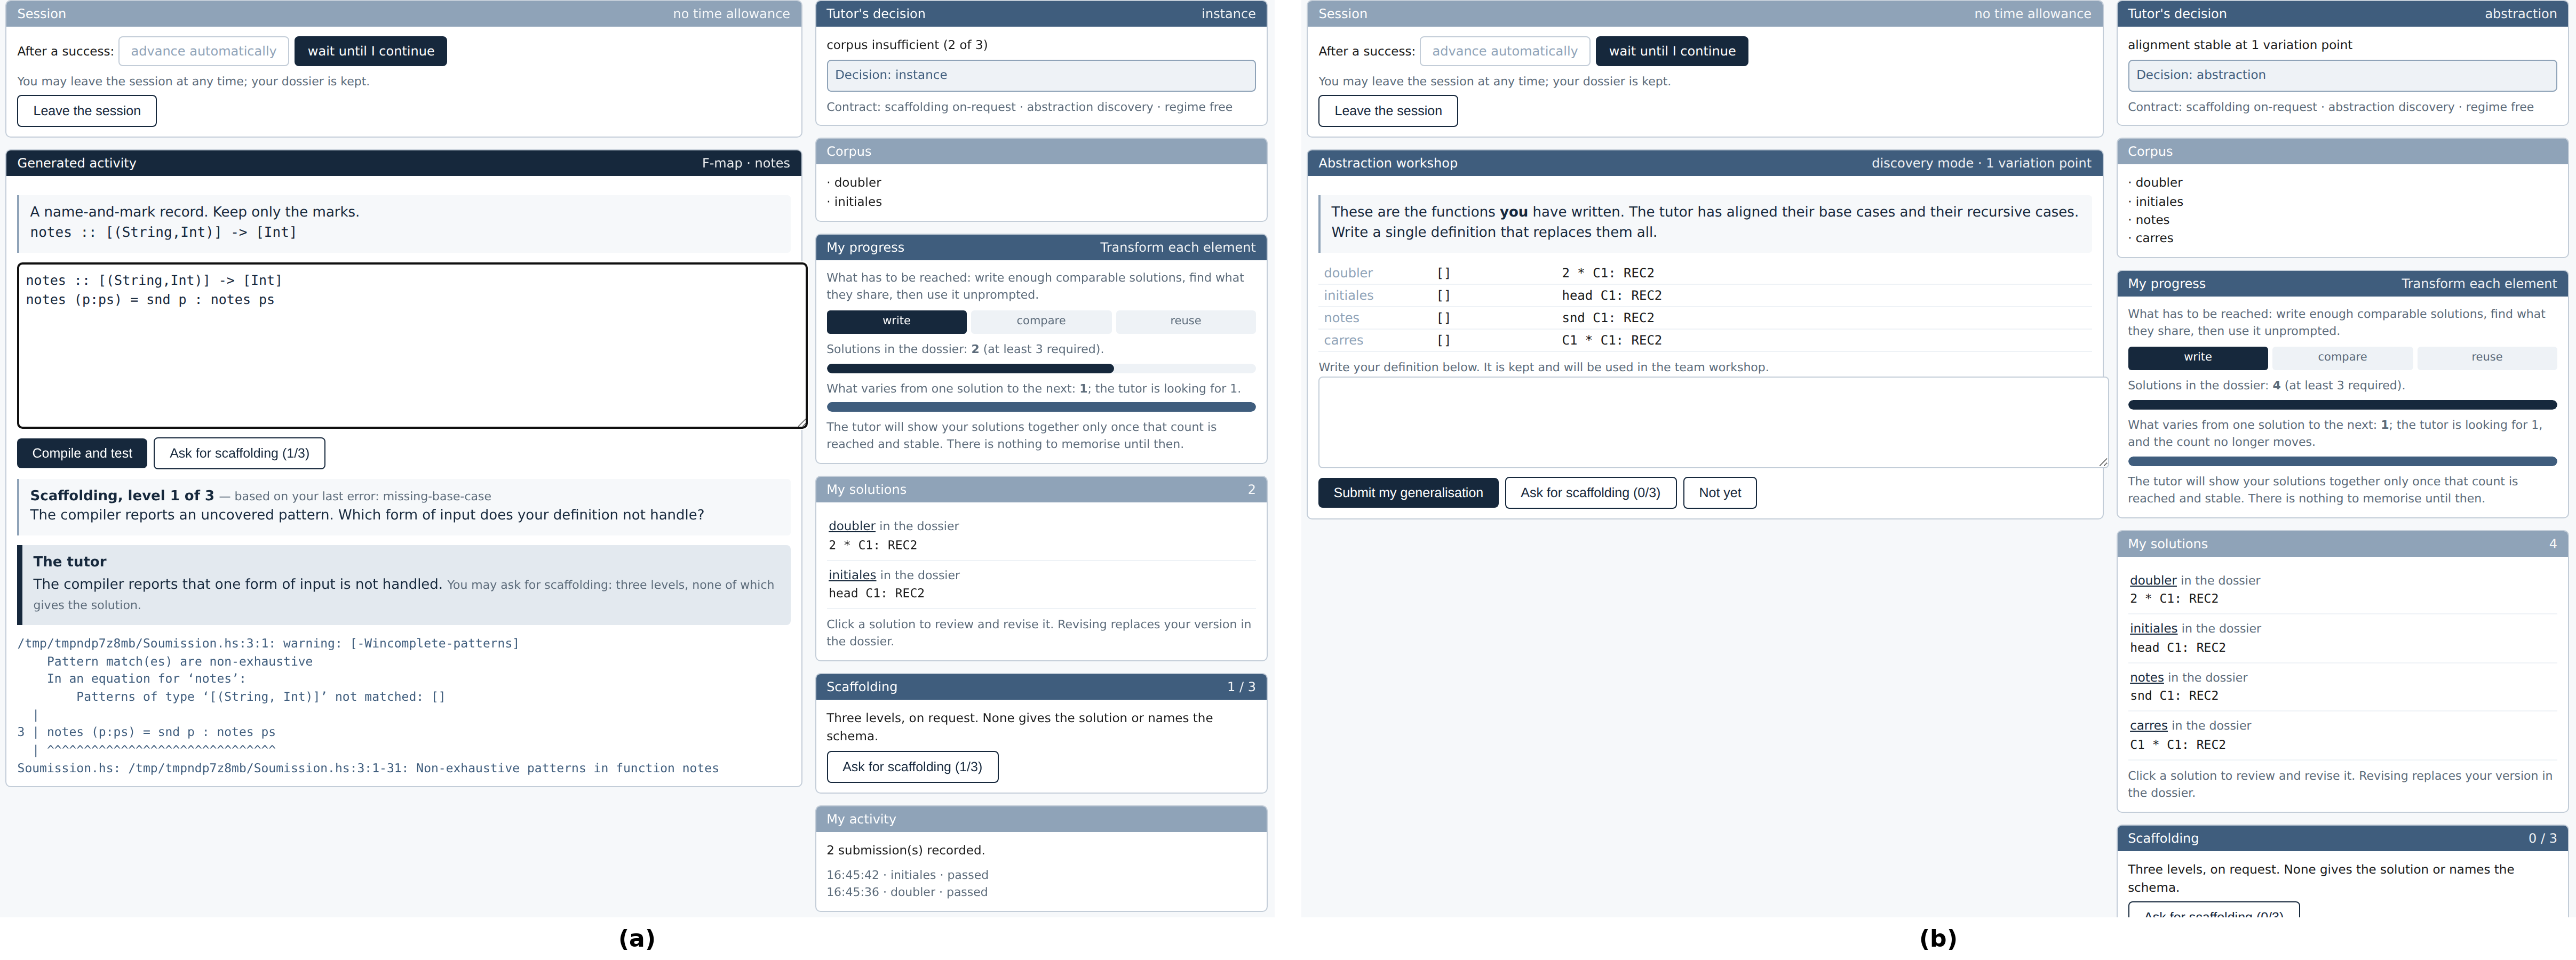
\includegraphics[width=\textwidth,height=3.30in,keepaspectratio]{fig1_haskell.png}
\caption{Two moments in a Haskell session, center and right panels of the learner's view. (a) The learner has submitted \texttt{notes (p:ps) = snd p : notes ps}, visible in the editor, which omits the equation for the empty list. The tutor gives a plain-language reading of the compiler message, the raw GHC warning appears below it, one level of scaffolding has been taken, and the progress panel reports two comparable solutions with one thing varying across them. (b) The abstraction workshop, opened once a fourth solution has confirmed the count, showing the learner's own four definitions aligned by base case and by step.}
\end{figure*}

Four elements of that view are consequences of the requirements above
rather than interface preferences. The workshop shows the learner's own
definitions and never canonical ones, since what distinguishes
productive failure from delayed exposition is that the consolidation
operates on what the learner produced. The progress panel reports how
many things currently vary across those definitions and how many the
tutor is seeking, which is a cue about the state of the knowledge rather
than a count of completed items. The scaffolding ladder has three levels
and none of them names the schema, since naming it early undoes the
purpose of the preceding activities. The tutor's decision appears with
its reason, including a refusal to trigger on a count that has reached the
target but has not yet been confirmed.

The response to a correct but non-comparable submission is where the
third requirement becomes visible. It is shown for the Python
instantiation in Fig. 5(a), so that the service can be seen after transfer
rather than before it.

\subsubsection{Teacher Control}
Every decision that carries a pedagogical commitment is a per-concept
contract, editable while the course runs (Fig. 2). Seven fields govern
scaffolding, the conduct of the abstraction, the work regime, whether a
sequence must be completed, a time allowance, the treatment of
non-comparable solutions, and the verification prompt.

\begin{figure*}[t]
\centering
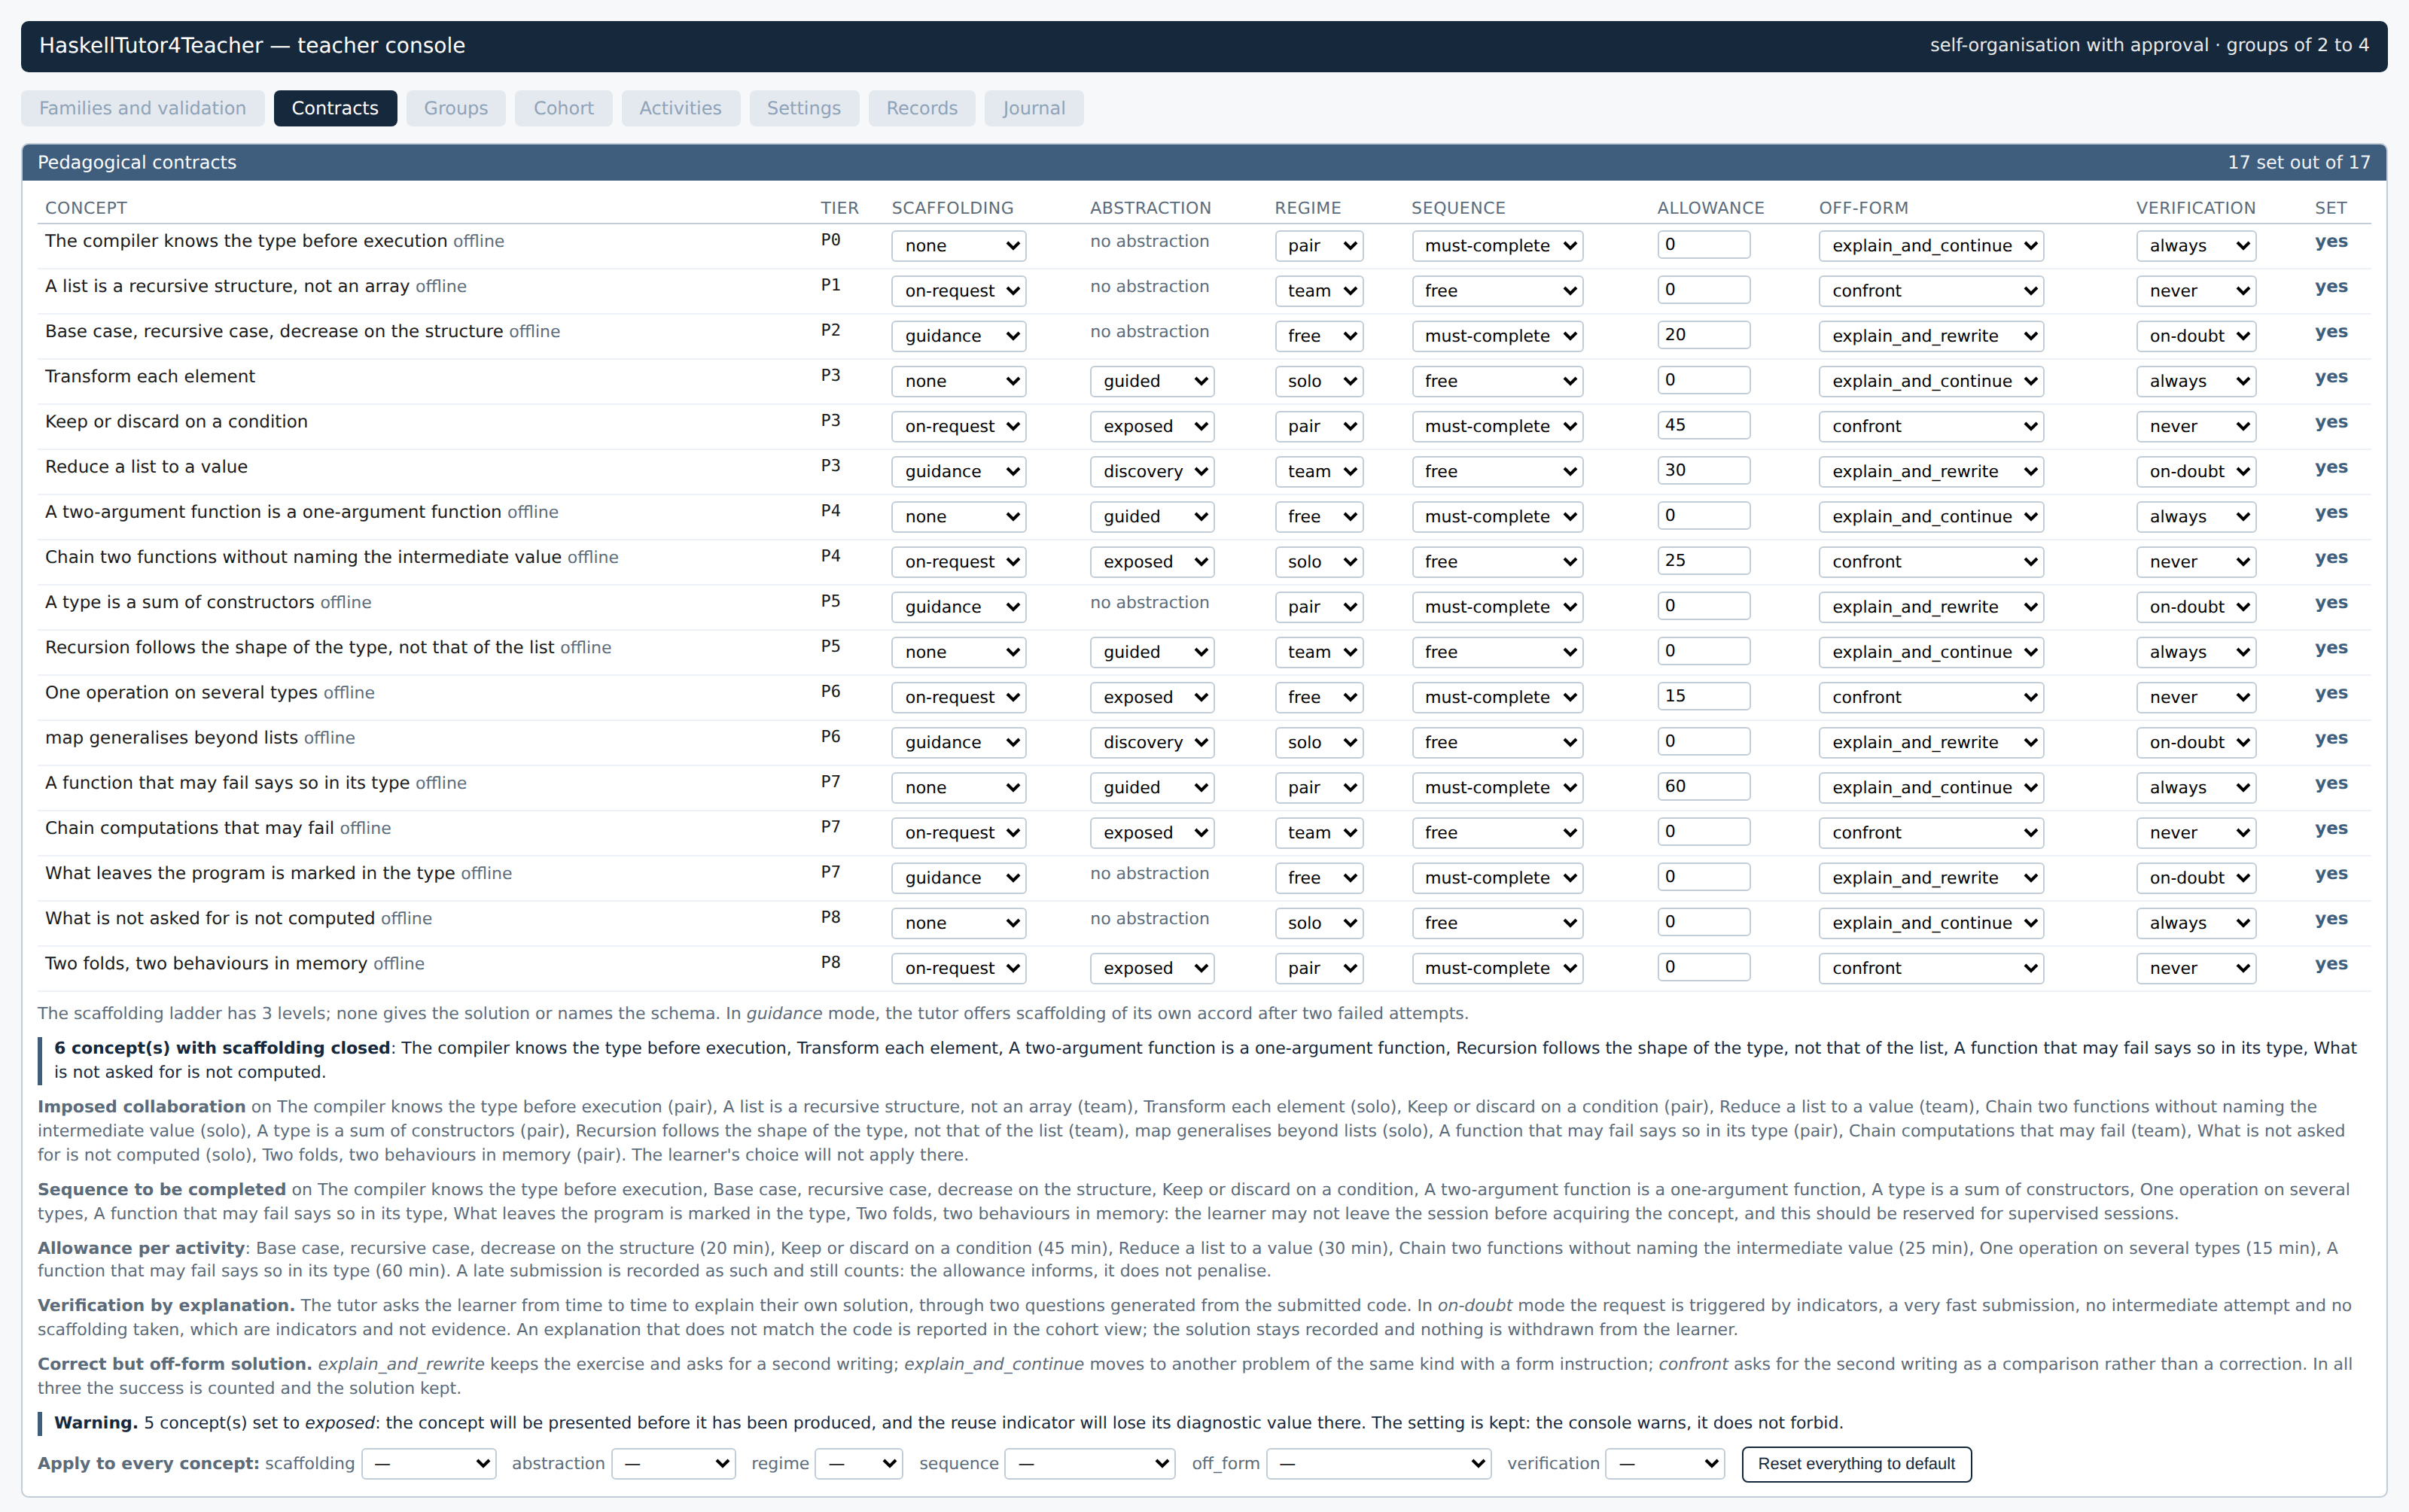
\includegraphics[width=\textwidth,height=3.45in,keepaspectratio]{fig4_contrats.png}
\caption{The contracts view, shown with settings deliberately varied across concepts so that the range of each field is visible. One row per concept, seven settings, applied immediately. Below the table, the console states what the current configuration costs: which concepts have scaffolding closed, which impose collaboration, which must be completed before the session can be left, which carry a time allowance, and which expose the schema and therefore lose the diagnostic value of the reuse indicator.}
\end{figure*}

Setting the abstraction field to \emph{exposed} converts a concept to
conventional exposition. The system applies the setting and states its
cost. This allows a teacher who is unconvinced by the default, or short
of time, to use the system rather than abandon it, and it allows the
comparison between instructional orders to be run inside a single
system.

Fig. 3 shows the family validation view, which is the teacher-facing
form of the first requirement.

\begin{figure*}[t]
\centering
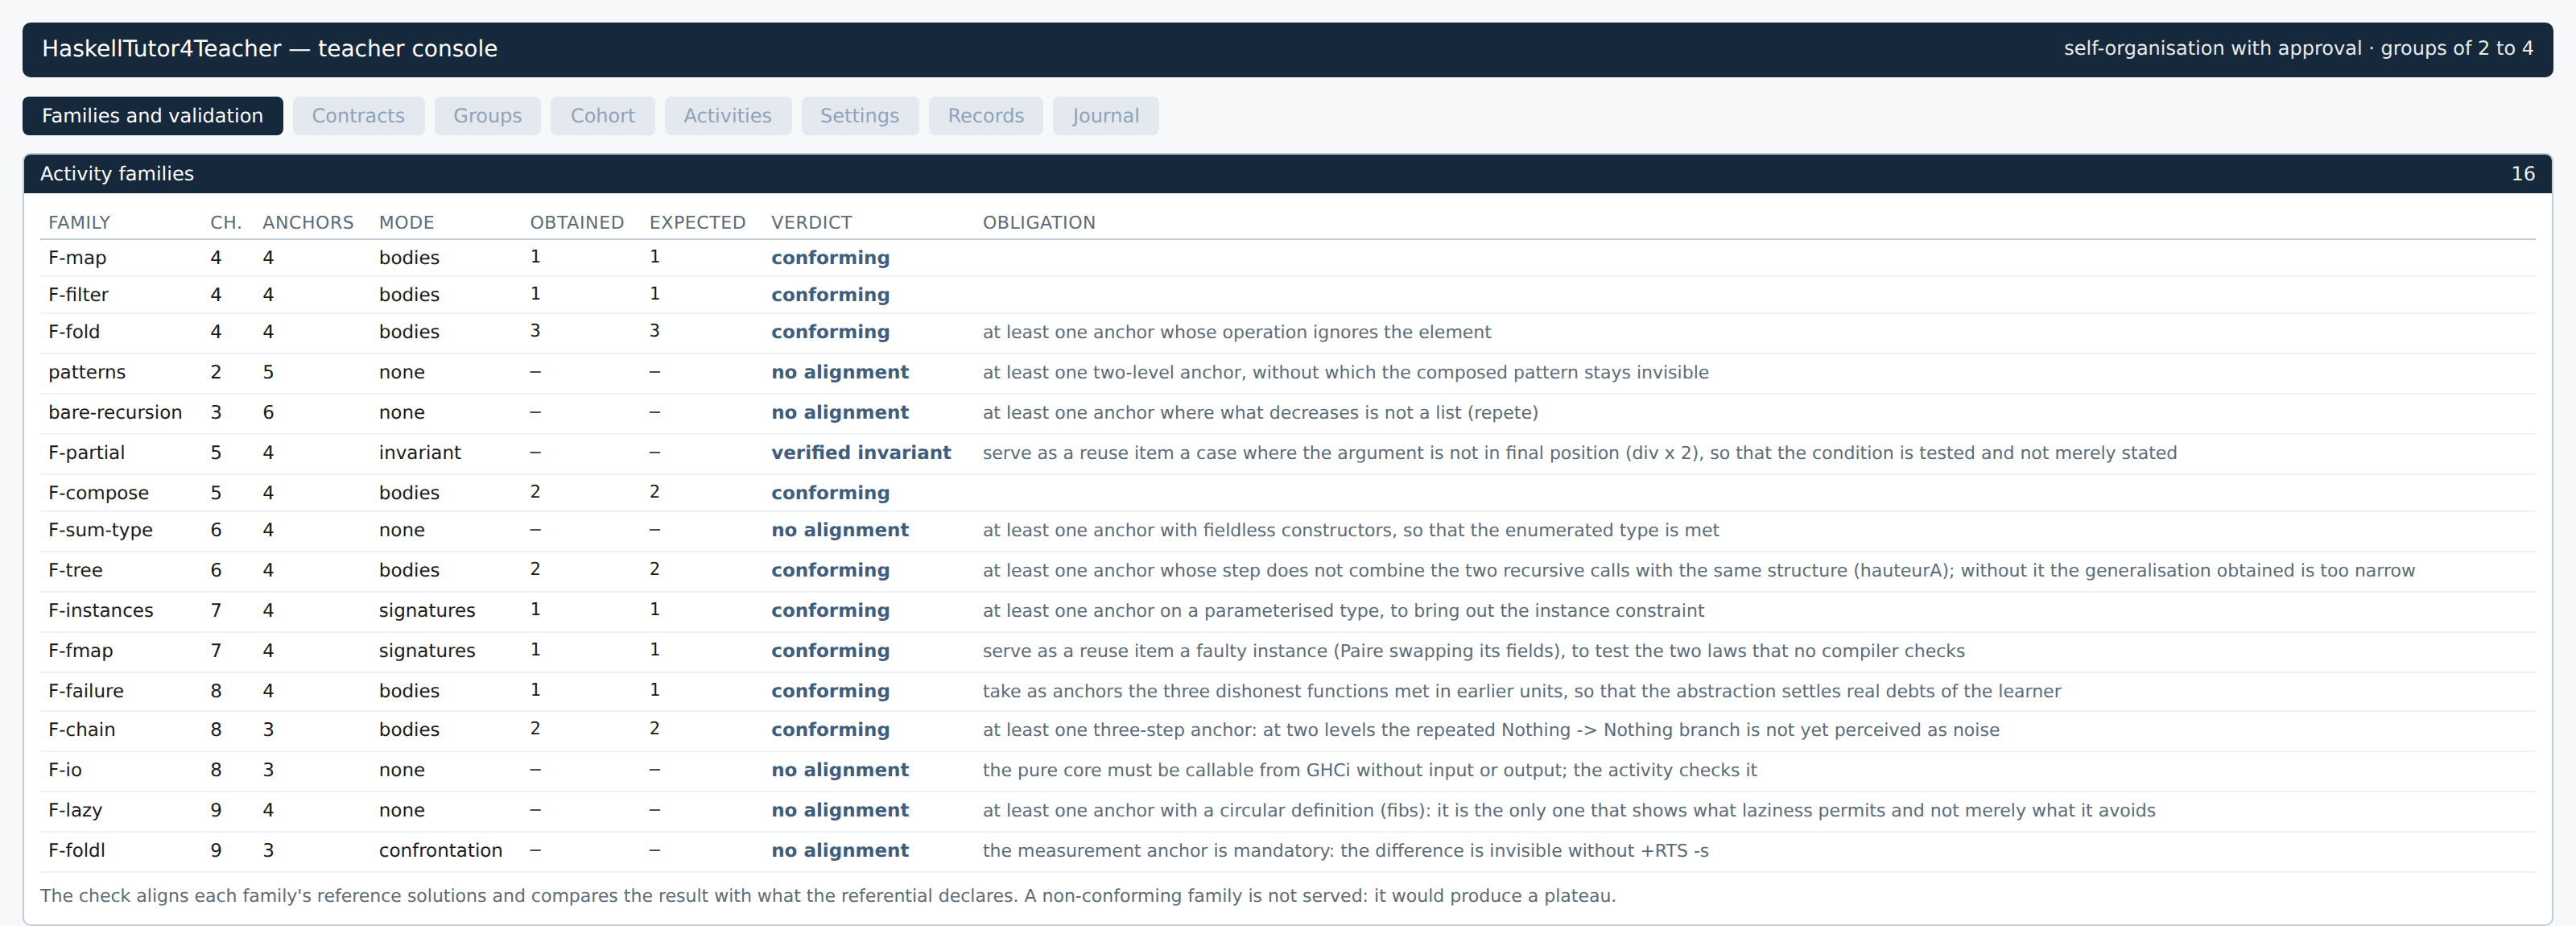
\includegraphics[width=\textwidth,height=3.60in,keepaspectratio]{fig2_familles.png}
\caption{Family validation. For each of the sixteen families: the course unit it serves (ch.), its anchors, its validation mode, the variation points obtained by aligning its own reference solutions, the number the referential declares, the verdict, and its obligation. A family that does not conform is not served.}
\end{figure*}

\subsubsection{The Case for Preservation}
Three arguments support preservation, and they do not carry equal
weight.

The weakest is cost. The decisions above took the better part of a year,
most of it spent failing. Reconstruction would cost something
comparable, and there is no particular reason to expect a second team to
take the same route.

The strongest is that these decisions cannot be seen by reading code,
and the ablation studies of Section 8 provide the evidence. Removing the
stability condition leaves a tutor that still triggers and a workshop
that still looks reasonable; it simply opens one solution early, in
every family measured. Removing the commutativity normalization leaves a
tutor that still aligns and that rejects solutions structurally
identical to ones it accepted. Removing the guard orientation rule
leaves a family that quietly fails to reach its target. None of these
failures announces itself. An author who had not encountered them would
attribute the symptoms to the difficulty of the material or to the
weakness of the cohort.

Between the two sits an argument from the authors' own experience. The
family validator, which encodes the first requirement, found three
defects in material that had been written and reviewed. The ablation
studies found a fourth, namely a normalization that had been present,
was lost in a rewrite, and was noticed by neither code review nor the
validator. A system built expressly to embody these commitments drifted
from them, which suggests that a system rebuilt from a description of
them would not embody them at all.

\section{Extraction Method and Measurement}
\subsection{Subtraction Rather Than Design}
The framework was not designed and then checked against the system. The
working system was taken as given, and everything that would not survive
a change of language was removed piece by piece, after which what
remained standing was examined.

A framework obtained this way contains what a first instantiation
actually used rather than what its designers imagine a second one will
need. The characteristic risk is the opposite one, namely preserving
accidents of the first system as though they were general. Section 3.4
reports two cases in which that happened and how they were detected.

\subsection{The Classification Question}
A single question was applied to each unit of code: if the language
taught were not Haskell, would this be rewritten?

Three answers were possible. If the answer was no, the unit belongs to
the framework, which was the common case. If the answer was yes but the
unit's inputs and outputs could be described without reference to any
language, the unit belongs to a provider and its signature belongs to
the interface. Evaluating a submission is of this kind, since the
command differs between languages but the instruction to compile a text
and compare its output with declared values does not. If the answer was
yes and the unit's interface was itself language-specific, a defect had
been found: something in the framework was reaching into the language,
and either the framework or the interface had to change.

The work proceeded from the outside in, since an outer layer that turns
out to be language-dependent invalidates the classification of
everything beneath it. The clients were examined first and were found to
name Haskell constructs only in activity statements and in the on-demand
explanations of the form requirement, both of which are content rather
than code. The session layer followed and contained no language
reference at all. The core layer was the only mixed one and was
classified statement by statement, since language dependence within a
single function was common. The recognition layer came last, since the
point of the exercise was to establish whether anti-unification could be
shared.

\subsection{Measurement}
Table 1 gives the distribution obtained on a working system of
approximately 2500 lines, excluding the roughly 1100 lines of the
interface layer.

\begin{table*}[t]
\centering\scriptsize
\caption{Language Dependence by Layer}
\begin{tabular}{@{}p{0.68in}p{3.47in}p{0.93in}p{1.61in}@{}}
\toprule
Layer & Components & Lines & Language-dependent \\
\midrule
Interface & learner client, teacher console & $\sim$1100 (HTML/JS) & 0 (statements are content) \\
Policy & session server, generator, records & $\sim$1300 & 0 \\
Recognition & anti-unifier & 250 & 3 (comments only) \\
Recognition & normalizer & 285 & all \\
Core & activities, evaluation, admission, policy, learner model & 647 & 40 \\
\bottomrule
\end{tabular}
\end{table*}

The forty lines in the core are the execution command, the test-module
template, and the error-classification table. The normalizer is
language-dependent by construction. Everything else held, including the
family model, the learner model, the four-decision policy with its
stability condition, the contracts, the scaffolding ladder, the
treatment of non-comparable solutions, the verification prompt, and the
collaboration arrangement. Fig. 4 shows the resulting layers.

This proportion was not expected. The explanation became apparent only
afterwards: the pedagogy reasons about relations between learner
solutions rather than about properties of a language. What varies across
a corpus, whether a count has stabilized, and whether a submission
exhibits a base case are questions about terms, and a term is a term.

\begin{figure}[t]
\centering
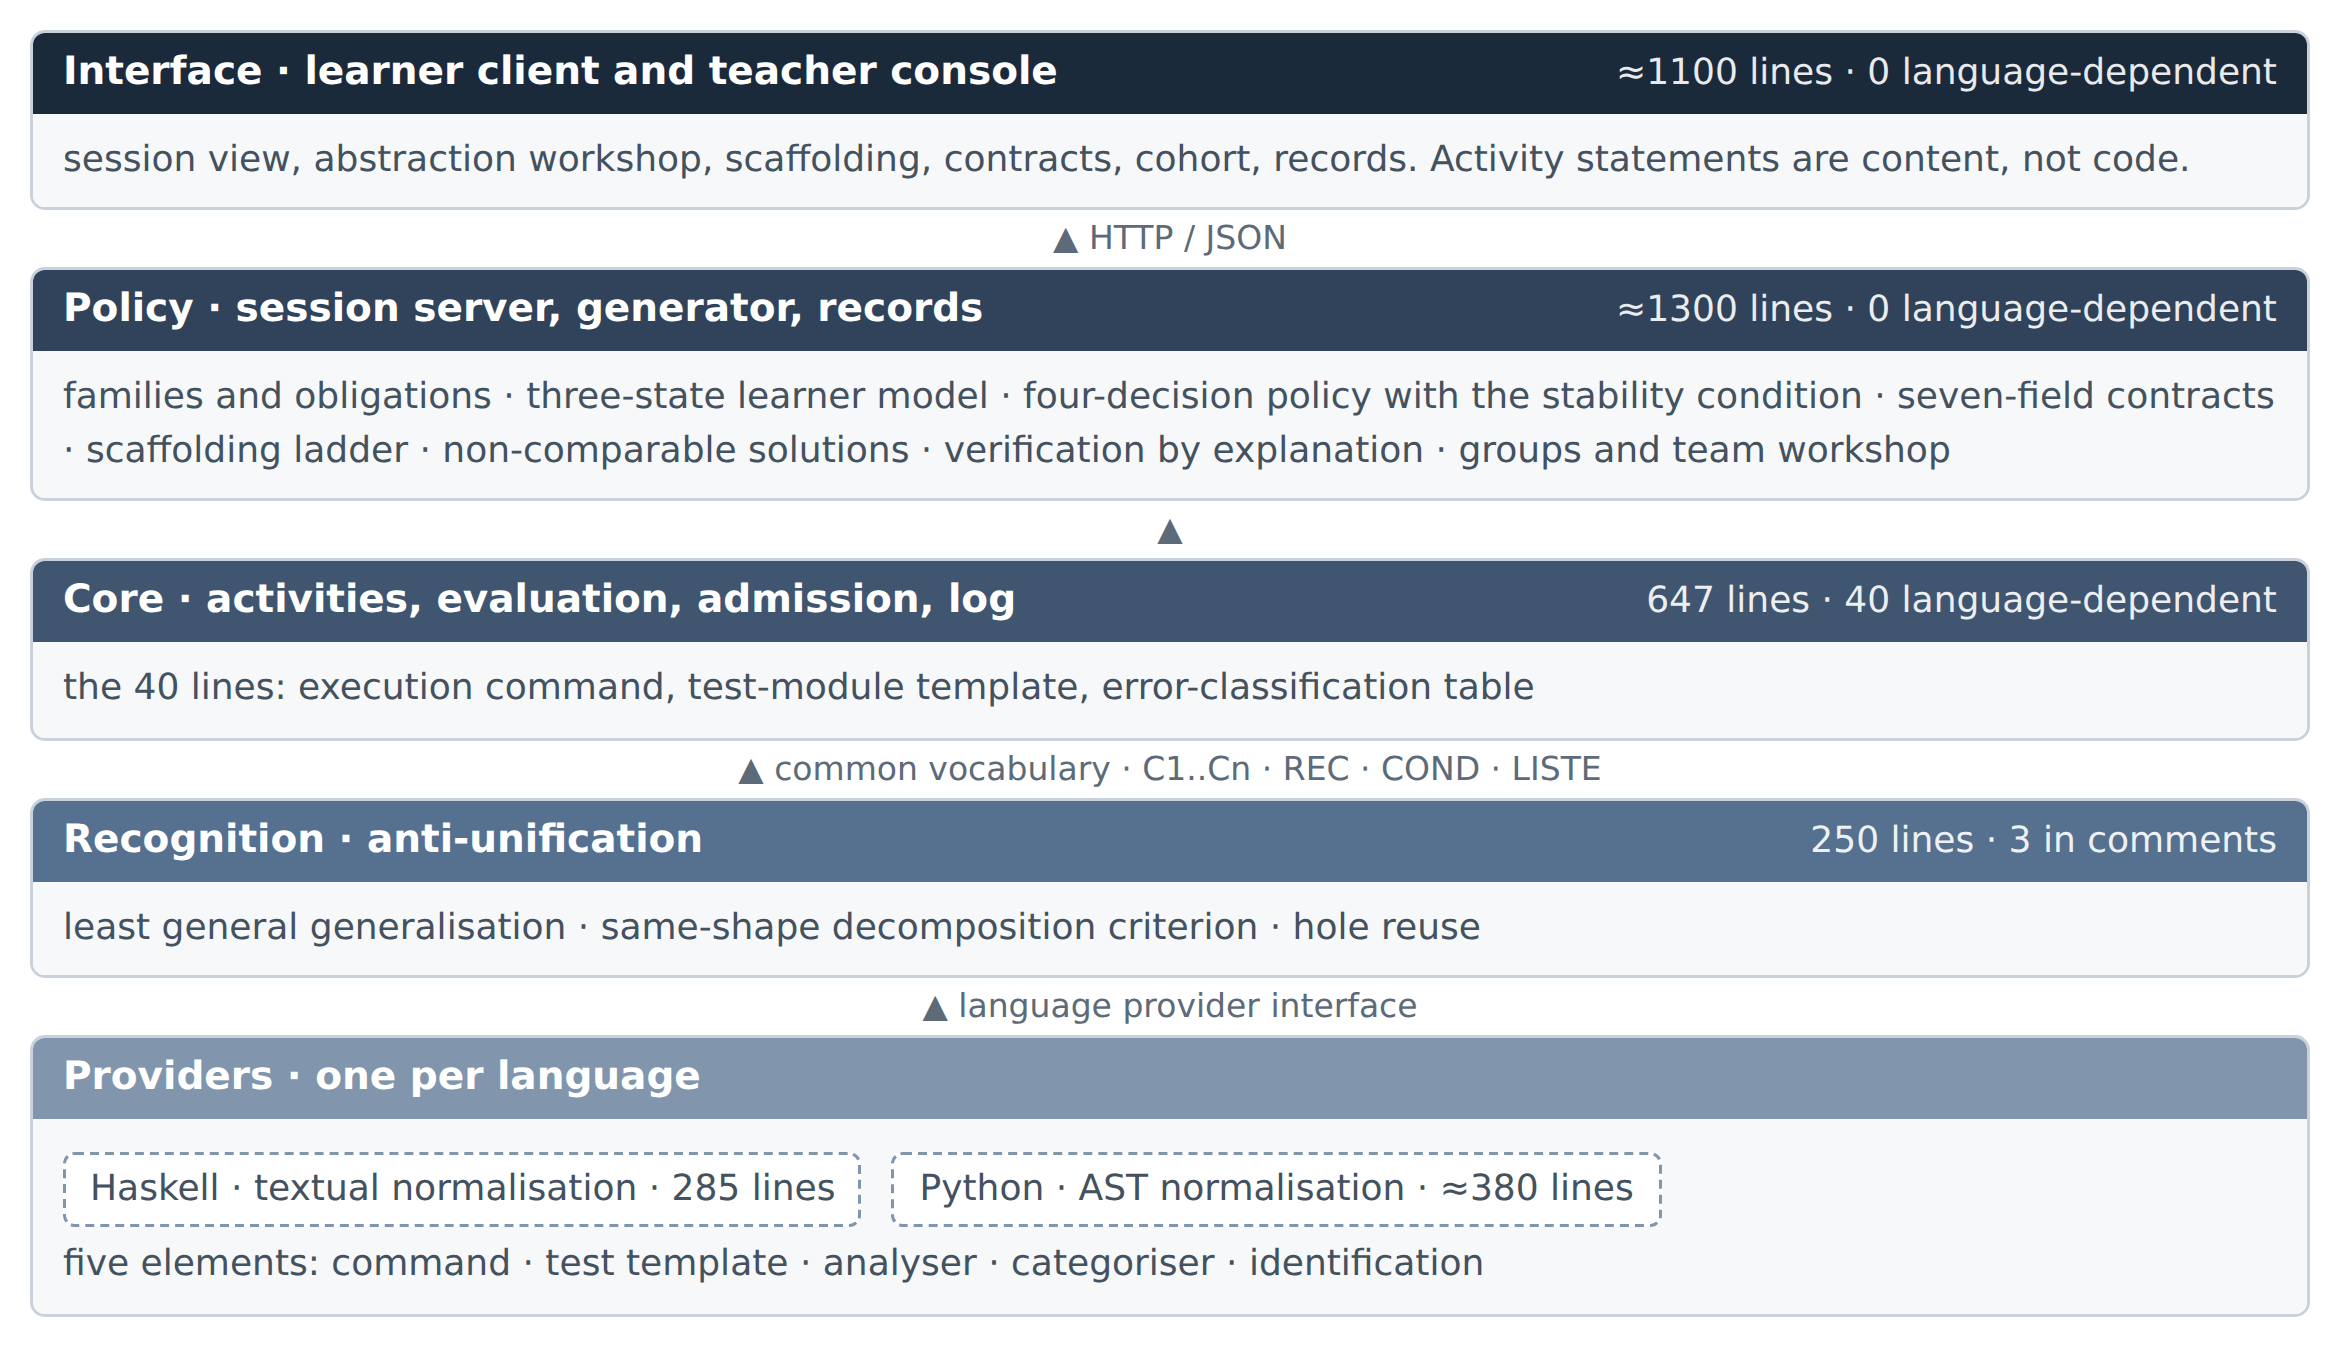
\includegraphics[width=\linewidth,height=2.40in,keepaspectratio]{fig_couches.png}
\caption{The layers after extraction, with their size and their language dependence. Everything above the provider interface is shared. A second language requires a provider with five elements.}
\end{figure}

\subsection{Two Interface Defects and One Missing Component}
Two components did not survive relocation and had to be redesigned.

The error classifier, which turns a compiler message into the first
level of scaffolding, had been written inline in the core as a chain of
tests on GHC message fragments. Being language-specific is not what made
it a defect. Its output was also language-specific, since the categories
were named after Haskell errors. The correction was to fix a common
vocabulary of categories, namely missing base case, incompatible types,
unknown name, syntax, and wrong result, and to have each provider map
its own messages onto it. The scaffolding ladder now consumes the
category and never sees the message.

The admission rule, which decides whether a correct submission may enter
the alignment corpus, had been expressed in terms of Haskell writing
styles. Correcting it meant having the analyser return one of a small
set of language-independent forms, namely constructors, no pattern,
iterative, no recursion, and unanalysable, and having the rule reason
over those. The correction paid off in an unplanned way: the Python
provider returns \emph{iterative} and \emph{comprehension}, categories
that do not exist in Haskell, and the admission rule handles them
unchanged, because it asks whether a form is admissible for a family
rather than what the form is called.

A third case illustrates the method's failure mode rather than a defect
it caught. The commutativity normalization, which makes
\texttt{x + f xs} and \texttt{f xs + x} coincide, was present in
the first normalizer and was lost when that module was rewritten.
Neither reading the code nor running the family validator revealed the
loss, because all reference solutions happen to be written in the same
operand order. It surfaced in the ablation study of Section 8.4, which
asks what changes when a component is removed and therefore also
answers, without being asked, whether the component is present.

\section{The Framework and Its Provider Interface}
\subsection{Elements Supplied by the Author}
Table 2 gives the interface in full.

\begin{table*}[h]
\centering\footnotesize
\caption{The Language Provider Interface}
\begin{tabular}{@{}p{1.05in}p{2.25in}p{2.4in}@{}}
\toprule
Element & Signature & Role \\
\midrule
\texttt{command} & path $\rightarrow$ argument list & run the test module \\
\texttt{test\_template} & code, expressions $\rightarrow$ source & assemble the test module \\
\texttt{analyse} & name, code $\rightarrow$ \{form, base, step\} & normalize to the common vocabulary \\
\texttt{categorise} & compiler message $\rightarrow$ category & first level of scaffolding \\
\texttt{name}, \texttt{extension} & strings & identification \\
\bottomrule
\end{tabular}
\end{table*}

Four of the five elements are trivial. The load falls on
\texttt{analyse}, and whether the framework is usable at all depends on
whether that function can be written by someone who did not build the
framework.

\subsection{The Common Vocabulary}
The interface is possible only because framework and providers share a
vocabulary belonging to neither language: \texttt{C1..Cn} for the fields
of a pattern, \texttt{REC} for a recursive call, \texttt{COND} for a
decision, \texttt{LISTE} for a list construction, and prefix application
for the rest. A provider expresses a learner's definition in those
terms, and the framework never looks inside them.

This is what allows the anti-unifier to be shared. Anti-unification
computes the least general generalization of a set of terms [18],
[19] and is indifferent to the language that produced them. In the
present case that is a measured fact rather than an aspiration, since
the 250-line module was used by the Python provider without
modification.

\subsection{Components Retained by the Framework}
The framework retains the activity family model with its variation axes,
prohibited axes, and obligations; the family validator; the three-state
learner model; the four-decision session policy, including the stability
condition and the instance ceiling; the contract layer; the three-level
scaffolding ladder; the treatment of correct but non-comparable
submissions and its three policies; the verification prompt; the
individual-then-confront collaboration arrangement; and the logging and
cohort reporting. An author supplies a provider, a set of anchors with
statements and tests, and a referential describing concepts and
families.

\section{Instantiation for Python}
\subsection{Rationale}
Python is the informative second case for three reasons. It is used
functionally in many introductory curricula, so the target schemas are
the same. It offers, for every list operation, at least four idioms,
namely comprehension, loop, \texttt{reduce}, and explicit recursion, of
which only the last is comparable in the sense the framework requires,
which places pressure on the treatment of non-comparable solutions. And
its standard library contains a parser, which proved more consequential
than expected.

\subsection{The Provider}
The Python provider is about 380 lines. Normalization is a walk over the tree
produced by the \texttt{ast} module, emitting the common vocabulary. A
subscript at index 0 on the function's parameter becomes \texttt{C1}, a
slice from index 1 becomes \texttt{RESTE}, a call to the function being
defined becomes \texttt{REC}, binary operators are emitted infix, and
method calls are emitted in prefix form so that
\texttt{xs[0].upper()} and \texttt{head x} acquire the same shape.

Two normalizations are semantic rather than syntactic and mirror the
Haskell provider. Commutativity applies to addition and multiplication
only, so that a step written \texttt{somme(xs[1:]) + xs[0]}
coincides with \texttt{xs[0] + somme(xs[1:])}; extending it to
concatenation would produce false identifications. The three ways of
writing the empty test, namely \texttt{not xs},
\texttt{len(xs) == 0}, and \texttt{xs == []}, are recognized as
one.

\subsection{Alignment Results}
Three Python definitions of the map family gave:
\begin{samepage}\noindent\begin{minipage}{\linewidth}
\begin{verbatim}
famille de transformation
  doubler     base []   pas ((LISTE (2 * C1)) + REC)
  majuscules  base []   pas ((LISTE (upper C1)) + REC)
  initiales   base []   pas ((LISTE (premier C1)) + REC)
  -> 1 point(s) de variation, attendu 1 : conforme
     forme ((LISTE ?1) + REC)
\end{verbatim}
\end{minipage}\end{samepage}


Four definitions of the fold family gave:
\begin{samepage}\noindent\begin{minipage}{\linewidth}
\begin{verbatim}
famille du pli
  somme       base 0    pas (C1 + REC)
  produit     base 1    pas (C1 * REC)
  longueur    base 0    pas (1 + REC)
  aplatir     base []   pas (C1 + REC)
  -> 3 point(s) de variation, attendu 3 : conforme
     forme (?2 ?1 REC)
\end{verbatim}
\end{minipage}\end{samepage}


These are the counts the Haskell instantiation produces for the
corresponding families, obtained by the same anti-unifier from canonical
forms generated by an entirely different normalizer. Both non-comparable
Python idioms are identified with a reason: the comprehension does not
expose the procedure, and the explicit loop has neither a base case nor
a recursive case.

\subsection{The Resulting Tutor}
\begin{figure*}[t]
\centering
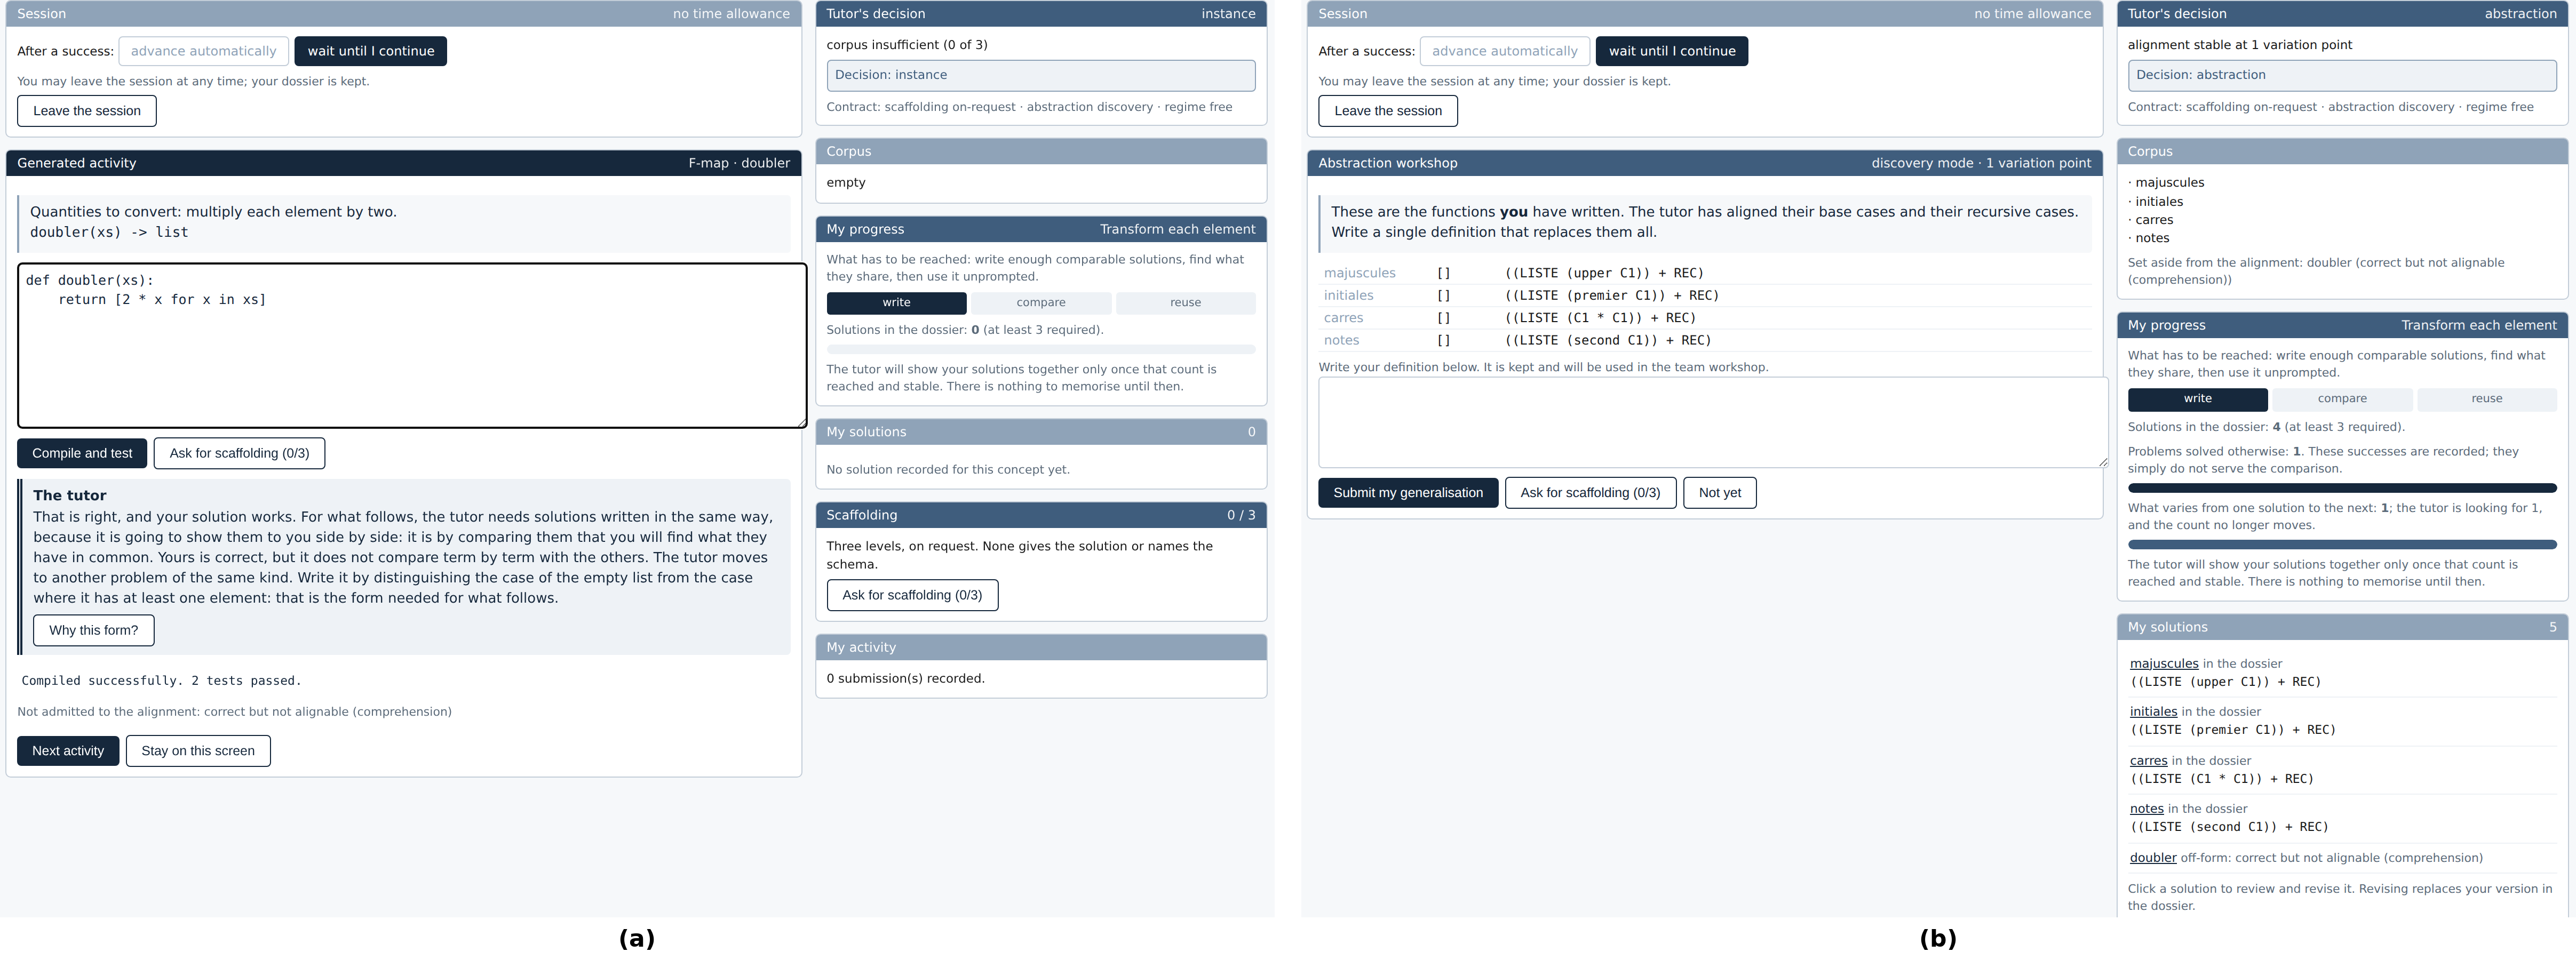
\includegraphics[width=\textwidth,height=3.30in,keepaspectratio]{fig5_python.png}
% Replace fig5_python.png with a capture after notes: the current image shows only three comparable definitions.
\caption{The same two moments in the Python instantiation. (a) The learner has submitted \texttt{return [2 * x for x in xs]}, visible in the editor. The code runs and passes both tests, and it cannot enter the comparison because it exhibits neither the base case nor the treatment of the head element. The tutor acknowledges the success, states what the comparison requires and why, offers the fuller explanation on request, and the corpus remains empty. (b) The abstraction workshop on four later definitions written by recursion, with the comprehension listed apart under the learner's solutions. Nothing in either view was rewritten for Python.}
\end{figure*}

Fig. 5 shows the learner-facing result: the same client, the same policy
layer, Python activities and Python code. Comparison with Fig. 1 is the
point of the figure. The two views differ in the code they contain and
in nothing else. The concept map, the
three-state progress display, the variation-point gauge, the record of
the learner's own solutions with their normalized forms, the scaffolding
counter, the pacing control, and the session suspension are all present,
and none was rewritten.

\subsection{An Interaction Sequence}
Fig. 5 shows the learner-facing states. The sequence below was reproduced
with the Python provider, activity set, referential, and corrected session
policy; all five submissions passed their executable tests.

The learner submits a list comprehension for the first activity. It
runs, passes both tests, and cannot enter the comparison. The tutor
acknowledges the success, records it in the separate register of
problems solved otherwise, states what the comparison requires and why,
and moves to another problem of the same kind with a form instruction
above the editor.

Two services visible in Fig. 5(a) are not properties of Haskell.
Classifying the submission as a comprehension rather than as
unanalysable comes from the Python provider, which recognizes the
construct, while the admission rule, which is framework code, consumes
that classification without knowing what a comprehension is. The
explanation of the requirement is the framework's, parameterized by
family rather than by language.

The learner then writes four explicit recursions, each admitted to the
corpus. The variation-point gauge can display a count after the second;
the session policy waits until the third before recording its first
count. The fourth confirms that count, and the workshop opens on the
learner's own four definitions. That is the framework's stability
condition operating on Python code. The
generalization she writes is stored, and under a collaborative contract
it would feed the team workshop.

The output of \texttt{trace\_pytutor.py} (Section 12), reproduced verbatim
except for line breaks, was:
\begin{samepage}\noindent\begin{minipage}{\linewidth}
\begin{verbatim}
minimum: 3
doubler: tests=ok, admission=no, corpus=0/3,
  points=None, decision=instance,
  reason=corpus insuffisant (0 sur 3)
majuscules: tests=ok, admission=yes, corpus=1/3,
  points=None, decision=instance,
  reason=corpus insuffisant (1 sur 3)
initiales: tests=ok, admission=yes, corpus=2/3,
  points=1, decision=instance,
  reason=corpus insuffisant (2 sur 3)
carres: tests=ok, admission=yes, corpus=3/3,
  points=1, decision=instance,
  reason=alignement a 1 points mais instable
notes: tests=ok, admission=yes, corpus=4/3,
  points=1, decision=remontee,
  reason=alignement stable a 1 points de variation
workshop corpus: majuscules, initiales, carres, notes
set aside: doubler
\end{verbatim}
\end{minipage}\end{samepage}


The comprehension consumed one of the Python family's five anchors,
leaving four comparable solutions. With only four anchors, the family
would have been exhausted after the first policy count, before a new
solution could confirm it; see Section 9.2.

\subsection{The Policy Layer}
The session policy was run on Python submissions by substituting the
provider and supplying Python anchors. As in Section 5.5, \texttt{doubler}
passes its tests but does not enter the alignment corpus. In the progress
label, ``of 3'' is the minimum before the policy evaluates alignment;
the display can calculate a count on two solutions, and a fourth
comparable solution confirms the policy's first count. The
\texttt{decision} and \texttt{reason} fields of the trace in Section 5.5 are
the policy's own output: \texttt{instance} with an insufficient corpus for
zero, one and two admitted solutions, \texttt{instance} with an unstable
alignment at three, and \texttt{remontee}, the system's label for the
abstraction decision, at four.



The policy's stability bookkeeping was corrected so that repeated reads
of an unchanged corpus cannot themselves confirm the count. The
parenthetical explanation after \texttt{doubler} describes its admission
status rather than the exact wording of a program log.

\section{Building a New Tutor}
The procedure below is the one followed for Python.

\textbf{Step 1: decide the target schemas and the concept graph.} The author writes the referential: concepts, prerequisites, and for each concept whether it is acquired through instances alone or through abstraction from a family. For Python the Haskell concept graph was kept unchanged, since the schemas are the same. An author teaching a different curriculum edits this file and nothing else.

\textbf{Step 2: write the provider.} The five elements. For Python this was about 380 lines, about 230 of them the analyser, and the work is a tree walk emitting the common vocabulary. One practical recommendation follows from experience: write the analyser against three or four reference solutions and print the canonical forms before connecting anything, since a canonical form that looks wrong on inspection is far cheaper to diagnose than an alignment count that comes out wrong two layers higher.

\textbf{Step 3: validate the provider on the test bench.} Supply writings known to be equivalent and writings known to be distinct. The Python provider failed this step on the first attempt in three ways, none of them visible by reading the code.

\textbf{Step 4: compose the families and let the tooling check them.} The author supplies reference solutions. The composition assistant reports the variation points obtained, and the obligation inducer reports which anchors are load-bearing. For the Python map family the inducer found every anchor interchangeable, in agreement with the Haskell instantiation of the same family.

\textbf{Step 5: write statements, stubs, and tests.} Template generation produces the stub and the test skeleton from the reference solution. The statement is the author's. This is the bulk of the remaining effort and the framework does not reduce it.

\textbf{Step 6: set the contracts and run.} For Python the non-comparable-solution policy would be set differently from Haskell, for reasons given in Section 9.2, and families would be sized one or two anchors larger.

A seventh step would be a classroom deployment. It has not been performed for Python and would exercise the parts of the procedure that a demonstration cannot, namely statement quality, family sizing, and contract choice.

\section{Authoring Tools}
A framework that exposes an interface and stops there moves the difficulty rather than reducing it. Three tools address the parts of authoring that proved expensive.

\subsection{Normalizer Test Bench}
A provider is validated against writings known to be equivalent. The bench runs them, confirms the equivalence claim, normalizes each, and reports the number of equivalence classes. A correct provider gives one class for syntactic variants and separate classes for semantically distinct writings.

\subsection{Obligation Inducer}
In the original system, obligations were found by hand while designing the activity families, at the point where the intended conclusion could not be justified from the anchors available. That took weeks and produced three obligations that were held with confidence, together with an unknown number that had been missed.

The operation is mechanizable. Align the complete family and record the count. Then, for each anchor, remove it, realign, and compare. An anchor whose removal changes the count is load-bearing, since it is the only member exhibiting one of the variations the family must display. The cost is linear in the number of anchors and each alignment is immediate. Table 3 reports the result on the five anchors of the fold family.

\begin{table*}[t]
\centering\scriptsize
\caption{Obligation Induction on the Fold Family}
\begin{tabular}{@{}p{1.07in}p{2.28in}p{1.34in}p{2.01in}@{}}
\toprule
Anchor & Points without it & Difference & Verdict \\
\midrule
somme & 3 & 0 & interchangeable \\
produit & 3 & 0 & interchangeable \\
longueur & 2 & $-$1 & \textbf{load-bearing} \\
aplatir & 3 & 0 & interchangeable \\
toutVrai & 3 & 0 & interchangeable \\
\bottomrule
\end{tabular}
\end{table*}

The induced obligation is the one that had been declared by hand, and
for the same reason: \texttt{longueur} is the only anchor whose
operation ignores the element, and without it learners conclude that the
combining function must consume the head.

The inducer also reports absence. For the map and filter
families it finds every anchor interchangeable, in agreement with the
referential, where neither family carries an obligation.

On the tree family it disagreed with the referential, informatively. It
names \texttt{listerA} where the referential names \texttt{hauteurA}, at
fine granularity as well as by blocks. \texttt{listerA} is the only
anchor whose base case differs: without it the base case no longer
varies, and the count falls from four points to two, or from two blocks
to one. \texttt{hauteurA} is the only anchor whose step does not combine
the two recursive calls with the same structure, but removing it leaves
the count unchanged, because the other anchors already make the step
vary. What changes is the generalized form, which becomes narrower,
\texttt{((?1 ?2 ?3) ?2 ?1)} instead of \texttt{(?4 ?2 ?1)}. Each anchor
therefore carries an obligation of a different kind. The hand-written
obligation named the one that protects the generality of the form and
missed the one that the count requires.

\subsection{Composition Assistant and Template Generation}
The composition assistant aligns an author's reference solutions,
reports the count, and flags degenerate families in which all anchors
share a property that was not intended to be shared. Template generation
produces the stub and test skeleton for an anchor from its reference
solution.

\section{Evaluation}
The evaluation is technical throughout: it asks what the framework
preserves when the language changes, not what learners gain from it.
Seven studies follow. Two establish that the extraction holds, four ablate
framework components in order to determine whether they are necessary, and
one ablates an author's anchors.
All are reproducible from the accompanying artefacts.

\subsection{Provider Correctness}
Seven writings of a summation in Python were used: four equivalent
structural recursions, differing in operand order, in the test for the
empty list, and in the use of a conditional expression, and three
distinct writings, namely a comprehension, a loop, and a library
function. The bench normalized each and reported the equivalence
classes.

On the first run the equivalent writings did not all coincide, and the
bench thereby located three defects. Commutativity was not applied, so that
\texttt{somme(xs[1:]) + xs[0]} did not coincide with
\texttt{xs[0] + somme(xs[1:])}. A \texttt{return} of a
conditional expression was not recognized as a base-and-step definition.
And a solution using a library function was classified as unanalysable
rather than as lacking recursion, which would have produced the wrong
explanation to the learner. After correction:
\begin{samepage}\noindent\begin{minipage}{\linewidth}
\begin{verbatim}
7 ecritures -> 4 terme(s) distinct(s)

  constructeurs  base 0        pas (C1 + REC)
      ordre direct, operandes echanges,
      test du vide autrement,
      expression conditionnelle
  comprehension  base -        pas -
      comprehension
  iteratif       base -        pas -
      boucle
  sans-recursion base -        pas (sum xs)
      fonction de bibliotheque

REUNION  ok : les 4 ecritures equivalentes rendent
  le meme terme.
SEPARATION ok : les 3 ecritures distinctes rendent
  des termes distincts.
\end{verbatim}
\end{minipage}\end{samepage}


\subsection{Agreement Between Instantiations}
On the map and fold families, compared in both languages, the counts agree: one
variation point for the map family and three for the fold family. The counts
are what the policy layer consumes, since the trigger compares them with
the family's declared target, so agreement here is what makes the shared
policy meaningful rather than coincidental.

\subsection{Ablation of the Decomposition Criterion}
When two subterms disagree, the engine must decide whether to decompose
the disagreement or generalize it as a block. Three policies were
compared on two-anchor prefixes of four families, which is where they
separate; with three or more anchors, hole reuse frequently collapses
the difference. Table 4 gives the resulting counts.

\begin{table*}[t]
\centering\scriptsize
\caption{Variation points under three decomposition policies. The counts are taken on two-anchor prefixes of each family, which is where the policies separate; this is why the fold family shows two points here and three in Section 5.3 and Table 7, where the complete family is aligned. The number in brackets after each family name is the count the retained criterion should give on that prefix.}
\begin{tabular}{@{}p{2.20in}p{0.95in}p{1.05in}p{0.85in}p{1.30in}@{}}
\toprule
Policy & filter (1) & composition (2) & fold (2) & map (1) \\
\midrule
Same-shape criterion (retained) & 1 $\checkmark$ & 2 $\checkmark$ & 2 $\checkmark$ & 1 $\checkmark$ \\
Always decompose & \textbf{2 $\times$} & 2 $\checkmark$ & 2 $\checkmark$ & 1 $\checkmark$ \\
Always generalize as a block & 1 $\checkmark$ & \textbf{1 $\times$} & 2 $\checkmark$ & 1 $\checkmark$ \\
\bottomrule
\end{tabular}
\end{table*}

Neither uniform policy serves all four families. Always decomposing
splits \texttt{even x} and \texttt{not (null x)} into a function
disagreement and an argument disagreement, where the pedagogically
correct reading is that the predicate as a whole is the single point of
variation. Always generalizing as a block collapses
\texttt{length (words s)} and \texttt{toUpper (head s)} into one
hole, where the correct reading is two. The retained criterion, which
decomposes when the disagreeing subterms have the same tree shape, is
the only one of the three that gives the intended count in all four
cases.

\subsection{Ablation of the Commutativity Normalization}
Three equivalent writings of a summation, differing in variable names
and in operand order, were used. Table 5 reports the metrics with and
without the normalization.

\begin{table}[h]
\centering\scriptsize
\caption{Configuration Metrics for Commutativity}
\begin{tabular}{@{}p{1.0in}p{0.9in}p{1.1in}@{}}
\toprule
Configuration & Equivalence classes & Canonical forms \\
\midrule
With commutativity & 1 & \texttt{C1 + REC2} \\
Without & 2 & \texttt{C1 + REC2}, \texttt{REC2 + C1} \\
\bottomrule
\end{tabular}
\end{table}

Without the normalization, a learner who writes the recursive call first
produces a submission that will not align with the others, and the tutor
sets aside a solution that is not merely correct but structurally
identical to ones it accepted.

This study also found the regression described in Section 3.4. The
component was absent from the current normalizer, having been lost in a
rewrite, and neither code review nor the family validator had noticed,
because every reference solution happens to be written in the same
order.

\subsection{Ablation of Guard Orientation}
Three definitions of the filter family were used, one of them written
with the negated guard and the branches exchanged, which is a writing
produced by a learner in the authors' trials. Table 6 reports the
metrics with and without orientation.

\begin{table}[h]
\centering\scriptsize
\caption{Configuration Metrics for Guard Orientation}
\begin{tabular}{lll}
\toprule
Configuration & Variation points & Generalized form \\
\midrule
With orientation & 1 (expected) & \texttt{COND ?1 (C1 : REC2) REC2} \\
Without & 2 & \texttt{COND ?3 ?2 ?2} \\
\bottomrule
\end{tabular}
\end{table}

Without orientation the family disperses. The tutor sees two points
where the target is one, declines to trigger, and continues serving
instances until the ceiling. The learner is penalized, without
explanation, for a writing choice that is semantically indistinguishable
from the accepted ones.

\subsection{Ablation of the Stability Condition}
The trigger requires that the alignment reach the family's expected
count and that the count be unchanged from the previous step. The effect
of the second conjunct was measured by building each family's corpus one
anchor at a time, and Table 7 gives the successive counts.
This ablation computes counts from two solutions to isolate the stability
condition; it is not a trace of the deployed session policy, whose
configured minimum is three.

\begin{table*}[t]
\centering\scriptsize
\caption{Successive Alignment Counts and the Effect of the Stability Condition. Counts begin with the second comparable solution; later entries correspond to successive admitted solutions.}
\begin{tabular}{@{}p{1.00in}p{0.55in}p{1.55in}p{1.85in}p{1.45in}@{}}
\toprule
Family & Expected & Counts as the corpus grows & Premature triggers without stability & Trigger with stability \\
\midrule
fold & 3 & 2, 3, 3, 3 & 1 & at the 4th solution \\
map & 1 & 1, 1, 1 & 1 & at the 3rd \\
filter & 1 & 1, 1, 1 & 1 & at the 3rd \\
failure & 1 & 1, 1 & 1 & at the 3rd \\
\bottomrule
\end{tabular}
\end{table*}

In every family the count reaches its target one step before it is
confirmed. A tutor without the condition therefore opens the abstraction
phase one solution early in every case measured. For the fold family
that is the difference between abstracting over three solutions and over
four, and since the third is the one that moves the count from two to
three, triggering immediately means triggering on a corpus whose
alignment has just changed.

The condition costs one comparable activity after the target count is first reached. Its effect is invisible
without this kind of measurement, since a tutor that triggers early
still triggers and still produces a plausible workshop. The pattern was
the same in all four families measured.

\subsection{Anchor Ablation and Obligation Induction}
The fifth study is the inducer of Section 7.2, whose results are not
repeated here. Its status differs from the three preceding studies.
Those ablate framework components in order to establish necessity,
whereas this one ablates content in order to establish a property of an
author's material. It is reported as an evaluation because it also
validates the framework: it recovers the obligation derived by hand on
the fold family, correctly reports absence on the map and filter
families, and on the tree family finds the obligation that had been
missed, while showing that the one declared by hand concerns the
generalized form rather than the count.

\subsection{Synthesis of the Evaluation}
Taken together, the seven studies support the claim of the paper: the
pedagogical components survive the change of language. The provider
interface was sufficient for a second language, the policy layer ran
unmodified, the alignment counts agreed, and the ablations show that the
components the framework retains are the ones it needs rather than
accidents of the first implementation. Section 11 states the boundaries
within which we make that claim.

\section{Discussion}
Three findings ran against expectation and are worth recording for
authors considering a similar extraction.

\subsection{Parser Availability and Instantiation Cost}
Python was expected to be harder than Haskell, since it offers more ways
to write the same computation. The two providers are of comparable size,
about 350 lines for Haskell and 380 for Python, even though the Python
provider recognizes more writings of each operation. The reason is that
the standard library
supplies a parser, which absorbs at no cost the writing variance, namely
parenthesization, spacing, identifier naming, and clause ordering, that
the Haskell provider handles textually and that was the part of the
original system needing the most repair. For an author choosing which
language to instantiate next, the operative question is whether a parser
exists in the implementation language rather than whether the target
language is simple.

\subsection{Inversion of Idiom Prevalence}
A Haskell learner asked for a list transformation usually writes
explicit recursion and occasionally a comprehension. In Python the
proportions reverse. The framework's treatment of correct but
non-comparable submissions, marginal in the first instantiation, becomes
the principal mechanism in the second.

Two consequences follow for an author. Families need more anchors, since
some will be consumed by non-comparable submissions; a four-anchor
map family would be exhausted before stability if one anchor were
consumed. The default policy should be \emph{confront}, which invites the learner to write a second, recursive solution alongside the correct but non-comparable one. Presenting the two writings as cases to compare,
rather than treating the first as an error to correct, gives the learner
an opportunity to discern what varies and what remains invariant
[20], and to notice distinctions before the shared structure is named
[21].

\subsection{Count, Form, and Granularity}
The disagreement reported in Section 7.2 shows that an obligation can
protect two different things. An anchor may be needed for the count to
reach the value the referential declares, which the inducer detects by
ablation, or for the generalized form to keep its generality, which the
count does not register. The inducer as specified covers the first kind.
The same ablations already expose the second: without \texttt{hauteurA}
the generalized form becomes narrower. Deciding which narrowings are
obligations requires a target, since removing \texttt{doubler} from the
map family also narrows the form, to a function applied to the element,
without the referential treating it as an obligation. The ablations
therefore allow structural obligations to be checked against an
explicitly specified target schema, which the referential already
declares for each family. Granularity raises a related
question for the session policy. The framework carries it as an explicit
field of a family, and the policy counts at the declared granularity.
This matters for the filter
family: when the admitted predicates share a shape, as comparisons do, the
fine count depends on the order and composition of the learner's corpus,
because the decomposition criterion of Section 8.3 splits predicates it
should treat as one. The filter family is therefore declared by blocks.
Replayed in all twenty-four orders of its four activities, it opens the
abstraction phase at the fourth solution in both instantiations. The general
observation is that mechanizing an instructional design tends to surface
the places where the design was underspecified, and that this is worth
expecting rather than being surprised by.

\section{Projections: A Neuro-Symbolic Architecture}
The material in this section is a projection rather than a result. Nothing described here has been implemented or measured, and we present it because the extraction reported above appears to have a consequence for the integration of large language models that is worth stating precisely.

The question the ITS community now faces is how to reconcile the fluidity of natural language interfaces with the structural commitments an instructional design makes. Prompting a generative model to act as a functional programming tutor is the direct approach, and it fails in a way that matters here. The model has no reason to withhold the name of a schema, and deferred exposure is the central commitment of the design we extracted.

The failure has a name. In earlier work [22] we defined a \emph{behavioral hallucination} as a case in which an agent claims adherence to a pedagogical theory but does not enact its defining principles, and showed that this can occur with no factual error at all: a tutor may give a correct solution while violating the commitment to learner exploration that it declares. Our measurements there indicate that prompt-level instruction does not sustain theory-consistent behavior over a multi-turn dialogue, and that the influence of an initial prompt attenuates as the conversation grows. The response proposed in that work is a runtime control layer that retrieves and operationalizes theory-based strategies during the interaction, which reduced the rate of behavioral hallucination substantially relative to a prompt-only baseline in a controlled simulation.

The situation here is a particular case of that one, and a favorable one. The commitment we need to protect is not a style of interaction but a single predicate over the learner's corpus: the name of a schema may be produced only after the alignment has stabilized at the count the family declares. Because that predicate is computable, it need not be retrieved, prompted or monitored. It can be enforced by refusing to make the phase available, which is what the framework already does for reasons that had nothing to do with generative models. Where PedRAG constrains a generative tutor at runtime with retrieved pedagogical strategies, the architecture sketched below constrains it by leaving the pedagogically consequential decision outside the model altogether. The two are complementary: most instructional commitments are not reducible to a computable predicate, and for those the runtime control of [22] remains the applicable instrument.

Reliability is the difficulty most often reported elsewhere as well. Hoq et al. [23] address it by keeping the instructor in the loop and by making the assistant's reasoning inspectable, which is another way of bounding a generative component. The interest of a decoupled architecture [24] is that it does not ask the model to respect that commitment.

\subsection{A Neural Provider}
The provider interface of Table 2 confines language dependence to five elements, of which only \texttt{analyse} is substantial. That element takes source text and returns a term in the common vocabulary. Nothing in the framework requires it to be written by hand.

A provider could therefore be driven by a language model constrained to emit a structured object, as sketched in Listing 1. The model would act as a translator from source text to schema rather than as a tutor, and the framework above it would be unchanged. If this worked, it would remove the requirement identified in Section 9.1, namely that a parser be available in the implementation language, and would allow instantiation for dialects or for pseudo-code. Algorithm 1 places such a provider in the ingestion loop, where only the parsing step is generative.

\begin{lstlisting}[float=htbp,basicstyle=\footnotesize\ttfamily,framexleftmargin=2pt,caption={Sketch of a neural provider constrained to the common vocabulary.}]
from pydantic import BaseModel, Field

class FormeCanonique(BaseModel):
    recursion_structurelle: bool = Field(
        description="True if the code is a base "
                    "case plus a recursive step.")
    cas_de_base: str = Field(
        description="Normalized base value.")
    cas_recursif: str = Field(
        description="Step in the common "
                    "vocabulary: C1, REC, COND, LISTE.")
\end{lstlisting}


\begin{algorithm}[t]
\SetAlgoLined
\DontPrintSemicolon
\footnotesize
\KwIn{learner submission $S$; family $F$; target variation points $V_{\mathrm{target}}$;
      count recorded at the previous step $C_{\mathrm{prev}}$}
\KwOut{action $A \in \{\textsc{OpenWorkshop},$ $\textsc{RetainConcept}, \textsc{ConfrontPolicy}\}$}
$E \leftarrow \textsc{RunTests}(S, F)$\;
\If{$\neg E.\mathit{passed}$}{\Return $\textsc{Scaffold}(E.\mathit{category})$\;}
\tcp{neural provider, constrained output}
$N \leftarrow \textsc{NeuralParser}(S, \mathit{schema} = \textsc{CanonicalForm})$\;
\tcp{symbolic layer from here on}
\If{$\neg N.\mathit{structural\_recursion}$}{\Return $\textsc{ConfrontPolicy}(F)$\;}
$\mathit{Corpus} \leftarrow \mathit{Corpus} \cup \{N.\mathit{step}\}$\;
$(G, C) \leftarrow \textsc{AntiUnify}(\mathit{Corpus})$\;
$\mathit{stable} \leftarrow (C = C_{\mathrm{prev}})$\;
\eIf{$C = V_{\mathrm{target}} \wedge \mathit{stable}$}{\Return $\textsc{OpenWorkshop}(G)$\;}
{$C_{\mathrm{prev}} \leftarrow C$\; \Return $\textsc{RetainConcept}()$\;}
\caption{Ingestion loop of the projected hybrid architecture. Only the parsing
step is generative; every decision below it is computed. The algorithm has not
been implemented.}
\end{algorithm}

\subsection{Conditions of Use}
The framework's guarantees rest on a property the present providers have and a language model does not: normalization is a function. Two writings that differ only syntactically must produce the same term every time, or the alignment counts on which the trigger depends become unstable. A model that returns \texttt{C1 + REC} on one call and \texttt{REC + C1} on the next would reproduce, at random, the failure documented in the ablation of Section 8.4.

Three checks would be needed before such a provider could be used. The test bench of Section 7.1 would have to be run as a gate rather than as a development aid, since it is exactly an instrument for detecting a normalizer that separates writings it should merge. Idempotence would have to be verified, by normalizing the same submission several times and requiring identical output. And agreement would have to be measured against a hand-written provider on a language where both exist, which is what our two instantiations make possible. We would not deploy a neural provider that had not passed all three, and we would expect the third to be the hard one.

A fourth question is what happens when the model returns nothing usable. A generative parser can fail in a way a hand-written one cannot: it may emit a structure that does not validate against the declared schema, or it may not answer in time. The response we would adopt treats such a failure exactly as the framework already treats a compilation failure. The symbolic layer catches the exception, the submission does not enter the corpus, and the session policy is asked for a decision with the submission marked as unevaluated, which is a state it already handles. What matters here is not the mechanism, which is ordinary, but where the boundary sits: a failure of the generative component reaches the learner as a tutor that could not evaluate a submission, and never as an abstraction phase opened on a corpus the framework did not verify.

\subsection{Symbolic Supervision}
What makes the projection interesting is not the provider but what sits above it. The policy layer, the anti-unifier, and the stability condition are algorithmic and would remain so. The decision to open the abstraction workshop would continue to follow from an alignment computed over the learner's corpus rather than from a model's judgment about readiness.

The stability condition would then act as a guardrail in a stronger sense than it does now. Its purpose in the present system is to avoid abstracting on a corpus that has not settled. In a hybrid system it would additionally bound what a generative component may cause to happen, since no amount of fluent interaction could open a phase that the alignment does not support.

\subsection{Learner-Facing Uses}
A generative component could also be placed in front of the learner rather than
behind the provider, as in the self-regulation support of Li and Ma [25], where a
model comments on the learner's process within a course context. That use is
attractive and it is not the one we would attempt first here, because the
commitment our design makes is precisely about what may be said to a learner and
when. The provider sits below the policy layer and never addresses the learner,
which is what makes it the safe place to start.

\subsection{Curriculum Co-Design}
The obligation inducer of Section 7.2 suggests a second use. It reports that a family lacks an exercise exhibiting a particular variation, and it identifies which variation. That is a precise specification, and writing an exercise to a precise specification is a task generative models perform reasonably well.

A plausible loop would have the inducer flag the gap, a model propose a statement with a reference solution and tests, and the framework validate the proposal by the same route it validates any other: run the tests, normalize the reference solution, realign the family, and check that the variation the proposal was meant to supply has appeared. A proposal that fails is discarded without a human seeing it. The check is the same one the framework already performs, which is what makes the loop safe rather than the model being reliable.

We record this as the most direct extension we can see, and note that it inverts the usual arrangement: the symbolic component is not a fallback for the model but the authority the model must satisfy.

\section{Conclusion and Future Work}
In this paper, a framework for building tutors that support bottom-up
abstraction in functional programming is proposed. It was obtained by
subtraction from a working system, and it was validated by instantiating
it for a second language. The results of our studies support the
following contributions.

First, the instructional design of such a tutor is largely independent
of the language taught. It occupies about eighty-five percent of the
implementation of HaskellTutor and contains no reference to Haskell,
because it reasons about relations between learner solutions rather than
about properties of a language. Language dependence concentrates in a
provider interface with five elements, of which one carries the load.

Second, the interface is sufficient for a second language of the same
paradigm. The Python provider is about 380 lines, it was connected to the
anti-unifier without modifying it, it reproduces the variation-point
counts of the Haskell instantiation on the two families tested, and the
session policy runs on Python submissions with no line changed.

Third, ablation is necessary to establish what a framework must retain.
Three components that had been added to solve particular problems proved
load-bearing in ways that could not be argued from inspection, and a
fourth study found a component that was no longer present. Subtraction
identifies what is language-independent; only ablation establishes what
is necessary.

Fourth, the most expensive part of the design can be mechanized. The
obligations of an activity family took us weeks to find by hand and were
found incompletely. An ablation over reference solutions recovers them
in seconds, including one exercise we had missed, and it exposes both the
obligations that the count requires and those that protect the form of
the generalization.

Finally, Section 10 sets out, as a projection rather than a result, what the same separation offers to a hybrid architecture. If the pedagogical policy is held apart from the domain knowledge, a language model can serve as a provider at the interface while the algebraic engine keeps the decisions that carry an instructional commitment. We have not built this system, and Section 10.2 states the conditions under which we would; we report it because the boundary the extraction produced turns out to be the boundary such an architecture needs.

Our study had several limitations. First, the framework targets
functional programming, Python included, and assumes the target family
is written by structural recursion with a base case and a recursive
case. It does not address imperative programming, where several
reasonable writings of one loop would align to a generalization so
general as to be uninformative. Normalizing to a control-flow skeleton
and aligning on execution traces were both considered, but neither is
implemented and neither should be assumed to work without trial. Second,
the Python instantiation is a demonstration rather than a deployed
tutor: it covers three families and fourteen activities, with statements
and tests written by us, and the studies of Section 8 compare two of
them. The agreement between instantiations reported in Section 8.2 rests
on those two families, the stability ablation of Section 8.6 on four,
and the provider test bench of Section 8.1 is small, whereas a released
framework would require a substantial bench per paradigm; we do not claim
that these results extend unexamined to larger families or to the
concepts not yet instantiated in both languages. The two recommendations
of Section 9.2 have not been tested with learners and are drawn from a
single instantiation.
Third, the procedure of Section 6 was carried out by the framework
designers, who knew where to look when a canonical form came out wrong;
the six steps are the ones an external author would follow, but the
effort we report for them is a lower bound. Fourth, the obligation inducer
operates on reference solutions the author supplies and inherits their
limits, since it can report that a family fails to exhibit a variation
but cannot report that a variation the author never considered is
missing; and it measures the count, so that an anchor needed only for the
generality of the form, such as \texttt{hauteurA}, is not reported as
load-bearing.

As future work, a third instantiation will be produced by an author
outside our group, working from the interface documentation alone, since
two instantiations by the same authors establish less than they appear
to. A full Python instantiation with a complete referential and
classroom use will follow, and will exercise the parts of the authoring
procedure that a demonstration cannot, namely statement quality, family
sizing, and contract choice. We also intend to test the two
recommendations of Section 9.2 with learners. The neural provider sketched in
Section 10 will be attempted only after the three checks described there
can be applied, since a normalizer that is not a function would
invalidate the guarantees on which the rest of the framework depends.

\section{Artefact Availability}
The framework, the Python instantiation, the Haskell normalizer with the
reference solutions of the families, the authoring tools, and the scripts
that reproduce every trace and technical study reported in this paper are
available at \url{https://github.com/nkambou/fptutor-shell2}. The scripts
require a Python~3 interpreter and no external library. Each result is
produced by a single command, run from the repository root:
\begin{verbatim}
# Section 5.3: alignments of the Python provider
(cd pytutor && python3 langue_python.py)
# Sections 5.5 and 5.6: Python session and policy
python3 trace_pytutor.py
# Section 8.1: provider test bench
(cd fptutor-shell && python3 banc_essai.py \
    --tuteur pytutor --cas cas_exemple.json \
    langue_python)
# Section 8.2: family validation, Haskell counts
python3 generateur.py
# Sections 8.3 to 8.6: Tables 4 to 7
python3 ablations.py
# Sections 7.2 and 8.7: Table 3
python3 obligations.py
\end{verbatim}
The interactive tutor shown in Figs. 1, 2, 3 and 5, with the Haskell and
Python providers, the learner interface and the teacher console, is
available at \url{https://github.com/nkambou/haskellTutor}; it requires
GHC for the Haskell provider. The provider interface of Table 2 is
documented in
\texttt{fptutor-shell/gabarit\_language.py}, which serves as the starting
point for a third instantiation.

\section*{Acknowledgments}
This work was supported by the Natural Sciences and Engineering Research
Council of Canada (NSERC) through a Discovery Grant.

\section*{References}
[1] W. van Melle, ``A domain-independent production-rule system for
consultation programs,'' in \emph{Proc. IJCAI}, 1979, pp. 923--925.

[2] T. Murray, ``Authoring intelligent tutoring systems: An analysis
of the state of the art,'' \emph{Int. J. Artif. Intell. Educ.}, vol. 10, pp. 98--129, 1999.

[3] T. Murray, S. Blessing, and S. Ainsworth, Eds., \emph{Authoring
Tools for Advanced Technology Learning Environments}. Dordrecht, The
Netherlands: Kluwer, 2003.

[4] V. Aleven, B. M. McLaren, J. Sewall, and K. R. Koedinger, ``A
new paradigm for intelligent tutoring systems: Example-tracing tutors,''
\emph{Int. J. Artif. Intell. Educ.}, vol. 19, no. 2,
pp. 105--154, 2009.

[5] A. Mitrovic, B. Martin, P. Suraweera, K. Zakharov, N. Milik, J.
Holland, and N. McGuigan, ``ASPIRE: An authoring system and deployment
environment for constraint-based tutors,'' \emph{Int. J. Artif. Intell. Educ.}, vol. 19, no. 2, pp. 155--188, 2009.

[6] R. A. Sottilare, K. W. Brawner, B. S. Goldberg, and H. K.
Holden, \emph{The Generalized Intelligent Framework for Tutoring
(GIFT)}. Orlando, FL, USA: U.S. Army Research Laboratory, 2012.

[7] R. Nkambou and A. Tato, ``Where the pedagogy lives outside the
code: A configurable tutor for functional programming, with bottom-up
abstraction as its default,'' 2026, submitted for publication.

[8] T. Cal\`o and C. J. MacLellan, ``Towards educator-driven tutor
authoring: Generative AI approaches for creating intelligent tutor
interfaces,'' in \emph{Proc. 11th ACM Conf. Learn. @ Scale (L@S '24)},
Atlanta, GA, USA, 2024, pp. 305--309, doi: 10.1145/3657604.3664694.

[9] Z. A. Pardos and S. Bhandari, ``ChatGPT-generated help produces
learning gains equivalent to human tutor-authored help on mathematics
skills,'' \emph{PLOS ONE}, vol. 19, no. 5, Art. no. e0304013, 2024.

[10] H. Keuning, B. Heeren, and J. Jeuring, ``Strategy-based feedback in
a programming tutor,'' in \emph{Proc. Computer Science Education Research
Conf. (CSERC '14)}, 2014, pp. 43--54.

[11] A. Gerdes, B. Heeren, J. Jeuring, and L. T. van Binsbergen,
``Ask-Elle: An adaptable programming tutor for Haskell giving automated
feedback,'' \emph{Int. J. Artif. Intell. Educ.}, vol. 27, no. 1,
pp. 65--100, 2017, doi: 10.1007/s40593-015-0080-x.

[12] A. N. Kumar, ``Solvelets: Tutors to practice the process of
programming,'' in \emph{Proc. 27th ACM Conf. Innov. Technol. Comput.
Sci. Educ. (ITiCSE 2022)}, Dublin, Ireland, 2022, pp. 151--157,
doi: 10.1145/3502718.3524811.

[13] B. Heeren and J. Jeuring, ``Feedback services for stepwise
exercises,'' \emph{Sci. Comput. Program.}, vol. 88, pp. 110--129, 2014, doi: 10.1016/j.scico.2014.02.021.

[14] K. Rivers and K. R. Koedinger, ``Data-driven hint generation in
vast solution spaces,'' \emph{Int. J. Artif. Intell. Educ.}, vol. 27, no. 1, pp. 37--64, 2017.

[15] T. W. Price, Y. Dong, and T. Barnes, ``Generating data-driven
hints for open-ended programming,'' in \emph{Proc. Int. Conf.
Educational Data Mining}, 2016.

[16] A. Deriyeva, J. Dannath, and B. Paa{\ss}en, ``SCRIPT: Implementing
an intelligent tutoring system for programming in a German university
context,'' in \emph{Proc. 26th Int. Conf. Artificial Intelligence in
Education (AIED 2025)}, Commun. Comput. Inf. Sci., vol. 2590. Cham,
Switzerland: Springer, 2025, pp. 168--177, doi: 10.1007/978-3-031-99261-2\_16.

[17] B. Kirouchenassamy, A. Yessad, S. Jolivet, and V. Luengo, ``Offline
reinforcement learning for adaptive feedback in online programming
education,'' in \emph{Proc. Int. Conf. Artificial Intelligence in
Education (AIED)}, Seoul, South Korea, 2026, pp. 79--93.

[18] G. D. Plotkin, ``A note on inductive generalization,''
\emph{Machine Intelligence}, vol. 5, pp. 153--163, 1970.

[19] J. C. Reynolds, ``Transformational systems and the algebraic
structure of atomic formulas,'' \emph{Machine Intelligence}, vol. 5,
pp. 135--151, 1970.

[20] F. Marton and M. F. Pang, ``On some necessary conditions of
learning,'' \emph{J. Learn. Sci.}, vol. 15, no. 2, pp. 193--220,
2006, doi: 10.1207/s15327809jls1502\_2.

[21] D. L. Schwartz and J. D. Bransford, ``A time for telling,''
\emph{Cogn. Instr.}, vol. 16, no. 4, pp. 475--522,
1998, doi: 10.1207/s1532690xci1604\_4.

[22] R. Nkambou, E. Nfor, and D. Kengne, ``PedRAG: Do LLM tutors
practice what they preach? Preventing behavioral hallucinations through
theory-grounded runtime control,'' in \emph{Proc. Int. Conf. Educational
Data Mining (EDM)}, 2026.

[23] M. Hoq, G. Pitts, B. Mott, S. Lee, J. Vandenberg, S. Jiao, N.
Norouzi, J. Lester, and B. Akram, ``An explainable AI assistant for
introductory programming education: Improving feedback reliability with
instructor-AI collaboration,'' in \emph{Proc. 27th Int. Conf. Artificial
Intelligence in Education (AIED 2026)}. Cham, Switzerland: Springer, 2026,
pp. 187--201, doi: 10.1007/978-3-032-29744-0\_13.

[24] M. K. Sarker, L. Zhou, A. Eberhart, and P. Hitzler,
``Neuro-symbolic artificial intelligence: Current trends, challenges, and
future directions,'' \emph{IEEE Intell. Syst.}, vol. 36, no. 6, pp.
75--81, 2021.

[25] H. Li and B. Ma, ``Design of AI-powered tool for self-regulation support
in programming education,'' presented at the CHI 2025 Workshop on Augmented
Educators and AI, Yokohama, Japan, 2025, arXiv:2504.03068.

\end{document}
